% !TeX program = pdflatex
\documentclass[11pt,a4paper]{article}
\usepackage[T1]{fontenc}
\usepackage[utf8]{inputenc}
\usepackage{amsmath,amssymb,amsthm,mathtools}
\usepackage{cite}
\IfFileExists{newtxtext.sty}{\usepackage{newtxtext,newtxmath}}{\usepackage{mathptmx}}
\usepackage{xcolor}
\newif\ifshowrevisions
% Default: black reading copy. Compile the revision wrapper for cumulative red.
\ifdefined\RevisionCopy\showrevisionstrue\else\showrevisionsfalse\fi
\newcommand{\rev}[1]{{\ifshowrevisions\color{red}\fi #1}}
\newenvironment{revision}{\par\begingroup\ifshowrevisions\color{red}\fi}{\par\endgroup}
\usepackage[margin=25mm,headheight=14pt,headsep=6mm,footskip=10mm]{geometry}
\usepackage{microtype,booktabs,array,tabularx,longtable,enumitem,needspace}
\renewcommand{\ttdefault}{pcr}
\usepackage{tikz,adjustbox}
\usetikzlibrary{arrows.meta,calc,patterns,positioning,shapes.geometric}
\usepackage{caption,float,placeins,flafter,fancyhdr,xurl}
\usepackage[hidelinks,bookmarksnumbered]{hyperref}
\pdfstringdefDisableCommands{\def\rev#1{#1}}
\newtheorem{theorem}{Theorem}[section]
\newtheorem{lemma}[theorem]{Lemma}
\newtheorem{proposition}[theorem]{Proposition}
\newtheorem{corollary}[theorem]{Corollary}
\theoremstyle{definition}
\newtheorem{assertion}[theorem]{Open assertion}
\newtheorem*{external}{External theorem}
\newtheorem*{remark}{Remark}
\newcommand{\Lconf}{\mathcal L}
\newcommand{\Pconf}{\mathcal P}
\newcommand{\Ttri}{\mathcal T}
\newcommand{\Z}{\mathbb Z}
\newcommand{\R}{\mathbb R}
\newcommand{\F}{\mathsf F}
\newcommand{\ind}{\mathbf1}
\newcommand{\spanA}{\operatorname{span}}
\newcommand{\mix}{B_{\mathrm{mix}}}
\newcommand{\force}{H_{\mathrm{force}}}
\newcolumntype{Y}{>{\raggedright\arraybackslash}X}
\setlist{nosep,leftmargin=1.5em,topsep=3pt}
\setlength{\parindent}{1.2em}
\setlength{\parskip}{0pt plus .3pt}
\makeatletter
\def\thm@space@setup{\thm@preskip=6pt plus 1pt\thm@postskip=6pt plus 1pt}
\makeatother
\setlength{\abovedisplayskip}{6pt plus 1pt minus 1pt}
\setlength{\belowdisplayskip}{6pt plus 1pt minus 1pt}
\setlength{\textfloatsep}{9pt plus 2pt}
\setlength{\intextsep}{9pt plus 2pt}
\setlength{\emergencystretch}{2em}
\captionsetup{font=small,labelfont=bf,skip=5pt}
\pagestyle{fancy}
\fancyhf{}
\fancyhead[L]{\small Additive energy and color forcing}
\fancyfoot[C]{\thepage}
\renewcommand{\headrulewidth}{.3pt}
\renewcommand{\sectionmark}[1]{\markboth{\thesection\quad #1}{\thesection\quad #1}}
\renewcommand{\topfraction}{.9}
\renewcommand{\bottomfraction}{.8}
\renewcommand{\textfraction}{.08}
\renewcommand{\floatpagefraction}{.75}
\numberwithin{equation}{section}
\urlstyle{same}
\hypersetup{pdftitle={Additive energy and color forcing in directed L-grid Ramsey problems},pdfauthor={Research collaboration}}
\begin{document}


\section*{Abstract}
\phantomsection\addcontentsline{toc}{section}{Abstract}
\begin{revision}
Two cells of the same color on the main diagonal of a grid force a third cell in a positive directed L to have another color. For an entire diagonal color class, all these restrictions must hold in a single coloring. We study their compatibility on the strict source
\[
V(A)=\{(v,u):u,v\in A,\ u<v\}
\]
of a finite integer set $A$. A proper two-coloring of $V(A)$ has no monochromatic triple $(x,y),(x+d,y),(x+d,y+d)$ with $d>0$.

Let $n=|A|$, put $M(A)=\binom n2$, and let $T(A)$ count these directed corners. If $r_d(A)=|\{u\in A:u+d\in A\}|$, then
\[
T(A)=\sum_{d>0}\binom{r_d(A)}2,
\qquad E(A)=2n^2-n+4T(A),
\]
where $E(A)$ is the additive energy. Thus repeated positive differences count the corner constraints. Bounding $T(A)$ would bound the number of mark pairs in terms of their span and hence constrain the original grid coloring. The difficulty is that several corners may share a completion cell, which must have the same color in all of them.

The first main result is a joint collision count for two disjoint Golomb sets $B,C$, each having no repeated positive difference. Writing $S=B\sqcup C$ and $\rho=|\Delta B\cap\Delta C|$, we prove
\[
T(S)\le\min\{2M(S),\ M(S)+5\rho\},
\]
with additional corrections for unequal class sizes. The proof counts collisions between the classes. Applied to the inherited fibers of a properly colored source, these estimates give local bounds. A forcing graph on the source cells records the compatibility constraints at shared completions. Controlling these constraints across the whole source remains necessary for a global bound.

We resolve two finite instances of the compatibility problem. The known binary Sidon capacity seven in dimension four excludes every injective five-dimensional Boolean cube from a properly two-colored strict source. A coloring of all $120$ cells of every separated four-cube shows that dimension four is attainable. For six-mark sets admitting proper source colorings, the exact maxima are $T=16$ and $E=130$. Every maximizing set is a translate and positive integer dilation of $\{0,1,2,3,4,6\}$ or its reflection. The proof combines an endpoint deficit, a complete attainment coloring, and a classification of the equality cases.

For several structured families, we obtain bounds for the whole source. Encoding graph edges as integers $5^i+5^j$ gives the exact identity $T(A_G)=2C_4(G)$, where four-cycles are unoriented and may have chords. Complete graphs show that any universal corner coefficient must be at least two. A separate probabilistic construction gives a family with no injective five-cubes for which no uniform linear corner bound holds. These sets are not shown to admit proper source colorings.

Full coloring certificates and finite verification records accompany the proofs. A uniform linear bound for arbitrary proper sources remains open. The numerical Ramsey consequences require explicit additional assumptions and give no new unconditional numerical bound.
\end{revision}
\medskip
\noindent\textbf{Keywords:} Ramsey theory, lattice colorings, additive energy, Golomb rulers, Boolean cubes.
\clearpage
\pdfbookmark[0]{Contents}{semifinal-contents}
\tableofcontents
\clearpage

\section{Introduction}\label{sec:introduction}
Write $[n]=\{1,\ldots,n\}$. A positive directed L is
\begin{equation}\label{eq:directed-L}
\Lconf(x,y;d)=\{(x,y),(x+d,y),(x+d,y+d)\},\qquad d\in\Z_{>0}.
\end{equation}
A coloring of a domain is \emph{proper} if no copy of \eqref{eq:directed-L} in that domain is monochromatic. Let $R_k(\Lconf)$ be the least $n$ for which $[n]^2$ has no proper coloring with $k$ colors. The legs have equal length and $d$ is positive.

If diagonal cells $(u,u)$ and $(v,v)$ share a color and $u<v$, properness excludes that color at $(v,u)$. Thus a proper coloring of the square restricts to a coloring with one fewer color on the strict source determined by any monochromatic diagonal class. Canakci et al.~\cite{CCFGMS23} and Mammel, Smith, and Yerger~\cite{MSY25} use this reduction in their bounds. We ask how many corners a finite integer set can support when a single proper two-coloring must cover its entire strict source.

For finite $A\subset\Z$, define
\begin{equation}\label{eq:source-notation}
\begin{gathered}
 V(A)=\{(v,u)\in A^2:u<v\},\qquad W(A)=\{(v,u)\in A^2:u\le v\},\\
 F_d(A)=\{u\in A:u+d\in A\},\qquad r_d(A)=|F_d(A)|\quad(d>0),\\
 n=|A|,\qquad M(A)=\binom n2,\qquad L(A)=\max A-\min A.
\end{gathered}
\end{equation}
We call $W(A)$ the weak source and set $L(\varnothing)=0$. The set $F_d(A)$ consists of the starts of cells with coordinate difference $d$. Write $T(A)$ for the number of directed corners in $V(A)$ and
$E(A)=\#\{(a,b,c,e)\in A^4:a-b=c-e\}$ for additive energy. Proposition~\ref{prop:counts} proves
\begin{equation}\label{eq:intro-counts}
 T(A)=\sum_{d>0}\binom{r_d(A)}2,
 \qquad E(A)=2n^2-n+4T(A).
\end{equation}
A \emph{Golomb set} has distinct positive differences. For any finite $B\subset\Z$, write $\Delta B=\{v-u:u,v\in B,\ u<v\}$. Each inherited fiber of a proper two-colored source splits into two Golomb classes. We count collisions between these classes, including the deficit from unequal sizes. A bound $T(A)\le CM(A)$ would imply $M(A)\le(1+2C)L(A)$ by Corollary~\ref{cor:span}, but no uniform $C$ is proved for arbitrary proper sources.

\begin{revision}
\paragraph{Research route.}
The Golomb restriction controls each color class within a fiber. To count the whole fiber, we must also count equal differences involving both classes. A second constraint arises between fibers: corners from different fibers may have the same completion cell, so their color requirements must agree there. We therefore combine a joint count for the two Golomb classes with a forcing graph on the source cells.

In a Boolean cube, each generator produces the same difference at many starts. A capacity bound on these starts obstructs a proper coloring, but attainment requires a coloring of every source cell. We also determine the six-mark maximum by proving an upper bound and specifying a coloring that attains it. For structured families, arithmetic and geometric relations allow a global count. In particular, the graph encoding identifies repeated pair sums with pairs of perfect matchings and hence with four-cycles.

The cube and six-mark results settle finite extremal questions. The structured estimates give linear bounds under their stated hypotheses. The random cube-free construction shows that cube exclusion alone cannot settle the general source problem. The forcing identity identifies the quantity that still needs a global bound. Until such a bound is proved, the numerical Ramsey consequences remain conditional.
\end{revision}

The density and Ramsey background comes from the corners theorem of Ajtai and Szemer\'edi~\cite{AS74} and the work of Graham and Solymosi~\cite{GS06}. For three colors, the cited bounds are $21\le R_3(\Lconf)\le493$~\cite{CCFGMS23,MSY25}. Lemma~\ref{lem:transpose} verifies the orientation transfer. The quantitative corners theorem of Jaber et al.~\cite{JLLOS25} yields a general asymptotic bound. Appendix~\ref{sec:general} proves the transfer to positive directed L's.

Sidon and Golomb theory supplies the local restrictions~\cite{OB04,D09,TV06}. Related Sidon partitions are studied in~\cite{ESR24}. Partitioning a set into two Golomb classes need not bound its difference multiplicities by two. Indeed, for $C=B+t$ with $t>L(B)$, the cross difference $t$ occurs $|B|$ times. The count must therefore include cross-class pairs. For Boolean cubes, the binary Sidon capacity in dimension four is the known value seven~\cite{OEIS309370,Wood05}. We use it to constrain colorings on actual source cells.

\begin{revision}
\begin{table}[!htbp]
\centering\small
\ifshowrevisions\color{red}\fi
\caption{\rev{Starting points and the statements developed in this manuscript}}
\label{tab:contribution-overview}
\begin{tabularx}{\textwidth}{@{}>{\raggedright\arraybackslash}p{.32\textwidth}Y@{}}
\toprule
Starting point & Statement developed here\\\midrule
Diagonal exclusion and Golomb restrictions on inherited color classes~\cite{CCFGMS23,MSY25}
& Joint collision counts and explicit deficits in Theorem~\ref{thm:energy} and Corollaries~\ref{cor:imbalance}--\ref{cor:moments}. A forcing identity on shared source cells in Theorem~\ref{thm:forcing}.\\[4pt]
Binary Sidon capacity $a(4)=7$~\cite{OEIS309370,Wood05}
& Exact attainable dimension four, and sharp three-cube mixed-corner cost nine under $2$-dissociation, in Corollary~\ref{cor:cube-threshold} and Theorem~\ref{thm:nine}.\\[4pt]
Classical energy maximum~\cite{Heg23}, source counts in Proposition~\ref{prop:counts}, and the supplied six-term progression obstruction in Lemma~\ref{lem:small}
& Exact six-mark proper-source maxima $T=16$ and $E=130$, all maximizing mark sets, and a complete fifteen-cell attainment certificate in Corollary~\ref{prop:six-point-extremal}.\\[4pt]
Classical simplex-edge and Johnson geometric configurations~\cite{Musin09,BSS12}
& Sharp corner coefficient two under a midpoint-multiplicity condition, and the graph identity $T=2C_4(G)$, in Theorems~\ref{thm:midpoint-three} and~\ref{thm:graph-source}.\\[4pt]
Diagonal reduction from square colorings to sources~\cite{CCFGMS23,MSY25}
& Explicit span-to-Ramsey implications under open assumptions in Section~\ref{sec:conditional}. No unconditional numerical improvement.\\\bottomrule
\end{tabularx}
\end{table}

The exact six-mark classification in Section~\ref{sec:six-mark-extremizers} also supplies an energy bound used in the product estimates. The product and two-distance results extend the method to structured sources. The graph encoding gives explicit proper colorings and forces any universal corner coefficient to be at least two. The forcing identity describes the compatibility problem that remains for arbitrary sources. 

Detailed comparisons with the cited inputs appear in Appendix~\ref{app:provenance}. The appendices give complete coloring arrays and finite verification records. These checks supplement the proofs of the general statements.
\end{revision}

\begin{revision}
Section~\ref{sec:formalism} sets up the source counts and inherited colorings. Sections~\ref{sec:energy}--\ref{sec:structured} develop the joint count, the cube and forcing arguments, and structured sources. Section~\ref{sec:conditional} separates the span-to-Ramsey implications from their open assumptions. Appendices~\ref{app:verification}--\ref{app:rainbow-theory} collect the full finite certificates, structured examples, rainbow counting arguments, and SAT encoding. Appendix~\ref{sec:general} gives the transfer of the external corners theorem, Appendix~\ref{app:provenance} identifies the mathematical starting points, and Appendix~\ref{app:endpoint} records the endpoint-deletion route.
\end{revision}
\FloatBarrier

\section{Background and orientation}\label{sec:background}
The papers on L-problems with few colors~\cite{CCFGMS23,MSY25} use
$\Pconf(x,y;d)=\{(x,y),(x,y+d),(x+d,y+d)\}$ with $d>0$.
The two orientations have the same Ramsey numbers.

\begin{lemma}[Transposition]\label{lem:transpose}
For every $n,k\ge1$, coordinate transposition gives a bijection between
proper $k$-colorings of $[n]^2$ for $\Lconf$ and for $\Pconf$.
Consequently, $R_k(\Lconf)=R_k(\Pconf)$.
\end{lemma}
\begin{proof}
The involution $\sigma(x,y)=(y,x)$ satisfies
$\sigma(\Lconf(x,y;d))=\Pconf(y,x;d)$ with the same positive step.
Pullback by $\sigma$ therefore preserves properness in both directions.
\end{proof}

Table~\ref{tab:w1} in Appendix~\ref{app:verification} gives a small example
from the coloring in~\cite[Figure~1]{CCFGMS23}. Its red diagonal excludes red from the
strict source. For $A=[4]$, the fiber sizes are
$3,2,1$, giving $M=6$, $T=4$, and $E=44$.

\section{Source counts and inherited colorings}\label{sec:formalism}
All mark sets are finite subsets of $\Z$. We use
$V(A)$, $W(A)$, $F_d(A)$, $r_d(A)$, $M(A)$, and $L(A)$ as defined in
Section~\ref{sec:introduction}, suppressing $A$ when it is fixed.
Empty sets and singletons are allowed, with span zero.
Sums over fiber offsets run over positive integers unless stated otherwise.
The offset $d$ of a source cell is $x-y$. The step
of a corner is its leg length.

\begin{revision}
Figure~\ref{fig:source-offset-step} distinguishes the offset of a fiber from the common leg length of its corners.
\begin{figure}[!htbp]
\centering
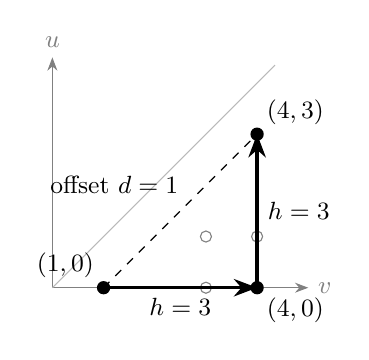
\begin{tikzpicture}[x=.65cm,y=.65cm,>=Stealth,every node/.style={font=\small},draw=black,text=black]
\draw[->,gray] (0,0)--(5.0,0) node[right] {$v$};
\draw[->,gray] (0,0)--(0,4.5) node[above] {$u$};
\draw[gray!55] (0,0)--(4.35,4.35);
\foreach \p in {(3,0),(3,1),(4,1)} \draw[gray,fill=white] \p circle(2pt);
\draw[dashed] (1,0)--(4,3) node[pos=.55,above left] {offset $d=1$};
\draw[->,very thick] (1,0)--(4,0) node[midway,below] {$h=3$};
\draw[->,very thick] (4,0)--(4,3) node[midway,right] {$h=3$};
\foreach \p in {(1,0),(4,0),(4,3)} \fill \p circle(2.4pt);
\node[above left] at (1,0) {$(1,0)$};
\node[below right] at (4,0) {$(4,0)$};
\node[above right] at (4,3) {$(4,3)$};
\end{tikzpicture}
\caption{\rev{The six strict-source cells for $A=\{0,1,3,4\}$. The bold legs join the parallel inputs $(1,0),(4,3)$ to their completion $(4,0)$. Both inputs have offset $d=1$, while the corner step is $h=3$.}}
\label{fig:source-offset-step}
\end{figure}
\end{revision}

\begin{proposition}[Exact source counts]\label{prop:counts}
For every finite $A\subset\Z$, with $n=|A|$,
\begin{equation}\label{eq:source-counts}
\begin{gathered}
\sum_{d>0}r_d=M,\qquad
T(A)=\sum_{d>0}\binom{r_d}{2},\\
\sum_{d>0}r_d^2=M+2T(A),\qquad
E(A)=2n^2-n+4T(A).
\end{gathered}
\end{equation}
The corners correspond bijectively to $d>0$ and $u<v$ in $F_d$, through
\begin{equation}\label{eq:source-corner}
(u+d,u),\quad(v+d,u),\quad(v+d,v).
\end{equation}
Their step is $v-u$.
\end{proposition}
\begin{proof}
Assigning each unordered pair of distinct marks its positive difference
gives $\sum r_d=M$. For $u<v$ in $F_d$, all four marks
$u,u+d,v,v+d$ lie in $A$, and the three cells in
\eqref{eq:source-corner} form a strict corner. Conversely,
$(x,y),(x+h,y),(x+h,y+h)$ determines
$u=y$, $v=y+h$, and $d=x-y>0$. The constructions are inverse
even when $u+d=v$, proving the formula for $T$.
The square-sum identity follows from $r^2=r+2\binom r2$.
Zero has $n$ ordered representations as a difference, while each
$d$ and $-d$ has $r_d$. Hence
$E=n^2+2\sum r_d^2=2n^2-n+4T$.
The same formulas hold for empty sets and singletons.
\end{proof}

The following restriction is the diagonal-exclusion mechanism
of~\cite[Theorem~2.3]{CCFGMS23} and~\cite[Theorem~2]{MSY25}.

\begin{lemma}[Diagonal exclusion and weak restriction]\label{lem:restriction}
Let $\chi:[N]^2\to[k]$ be proper and suppose
$\chi(a,a)=c_0$ for every $a\in A\subseteq[N]$.
Then $\chi|_{V(A)}$ is proper and avoids $c_0$.
More generally, if $z:V(A)\to\Omega$ is proper, then for every $d>0$,
\begin{equation}\label{eq:weak-restriction}
w_d(v,u)=z(v+d,u),\qquad u,v\in F_d,\quad u\le v,
\end{equation}
defines a proper coloring of $W(F_d)$. Its diagonal color at $u$ is
$z(u+d,u)$.
\end{lemma}
\begin{proof}
For $u<v$ in $A$, the cells $(u,u),(v,u),(v,v)$ form a corner.
Its diagonal cells have color $c_0$, so $(v,u)$ has another color.
In \eqref{eq:weak-restriction}, $u,v\in F_d$ give
$u,v+d\in A$ and $v+d>u$, so the right-hand side is defined.
The map $(v,u)\mapsto(v+d,u)$ sends $W(F_d)$ into $V(A)$ and preserves
corners. A monochromatic corner in $w_d$ would therefore contradict
properness of $z$.
\end{proof}

We use the Golomb restriction of~\cite[proof of Theorem~6]{MSY25}.
A Golomb set has no repeated positive difference or, equivalently, no
repeated unordered pair sum, including doubled marks
\cite{OB04,D09}.

\begin{lemma}[Golomb classes and pair sums]\label{lem:golomb}
If $w:W(S)\to\{0,1\}$ is proper, each diagonal class
$B_i=\{a\in S:w(a,a)=i\}$ is Golomb.
Consequently, for a proper $z:V(A)\to\{0,1\}$, each
$B_{d,i}=\{u\in F_d:z(u+d,u)=i\}$ is Golomb.
In a Golomb set $B$, equality $b_1+b_2=b_3+b_4$ implies equality
of the unordered pairs with repetition.
\end{lemma}
\begin{proof}
Diagonal exclusion gives $w(v,u)=1-i$ whenever $u<v$ lie in $B_i$.
If $(a,a+h)$ and $(a+t,a+t+h)$ were distinct equal-difference pairs
in $B_i$, choose their order so that $h,t>0$.
The three strict cells
$(a+h,a),(a+t+h,a),(a+t+h,a+t)$ would all have color $1-i$ and form
a step-$t$ corner. Hence $B_i$ is Golomb.
Apply Lemma~\ref{lem:restriction} to obtain the fiber assertion.

For the pair-sum assertion, order each pair increasingly.
If the pairs differ, interchange them so that $b_1<b_3$.
Then $b_4<b_2$ and $b_3-b_1=b_2-b_4>0$.
The two difference pairs are distinct, since equality would force
$b_1=b_4\ge b_3$. This contradicts Golombness even if one pair
contains a repeated mark.
\end{proof}

\begin{corollary}[Energy to span]\label{cor:span}
If $T(A)\le\kappa M(A)$ for a finite $A\subset\Z$ and $\kappa\ge0$, then
\begin{equation}\label{eq:energy-to-span}
M(A)\le(2\kappa+1)L(A),\qquad
|A|\le\frac{1+\sqrt{1+8(2\kappa+1)L(A)}}2.
\end{equation}
In particular, $|A|\le1+\sqrt{2(2\kappa+1)L(A)}$.
\end{corollary}
\begin{proof}
If $M=0$, then $|A|\le1$ and the bounds hold.
Otherwise $L\ge1$, and the positive differences lie in $[L]$.
Cauchy--Schwarz and \eqref{eq:source-counts} give
$M^2\le L\sum_{d=1}^Lr_d^2=L(M+2T)\le(2\kappa+1)LM$.
Divide by $M>0$, then solve $n(n-1)\le2(2\kappa+1)L$ for $n$.
The final estimate follows from $(n-1)^2\le n(n-1)$ for $n\ge1$.
\end{proof}

\section{Two-Golomb energy and its limits}\label{sec:energy}
Each fiber of a proper strict two-coloring splits into two Golomb classes.
Differences represented by cross-class pairs may repeat. We distinguish these
representations by the class of the smaller mark.

For comparison with mixed additive energy~\cite[Section~2.1]{Cilleruelo10},
define $\mathcal E(B,C)$ to be the number of ordered solutions of
$b_1+c_1=b_2+c_2$ in $B\times C\times B\times C$.
For Golomb classes of sizes $b,c$, rearranging this equality gives
\begin{equation}\label{eq:mixed-energy-rho}
\mathcal E(B,C)=bc+2\rho,\qquad \rho=|\Delta B\cap\Delta C|.
\end{equation}
The zero difference contributes $bc$, and every shared positive difference
contributes once with each sign. These are ordered counts, unlike the
unordered counts in generalized Sidon conditions~\cite{CRV10}.

\begin{revision}
\medskip\noindent\textbf{The counting mechanism.}
Golombness controls pairs within each class, but a repeated difference can
also use cross-class pairs. To see the distinction, take
\[
B=\{0,2,5,6\},\qquad C=\{1,3,4,8\}.
\]
The cross pairs $3\to5$ and $4\to6$ both point from $C$ to $B$ and
have length two. Their starts and ends give the internal pairs
$\{3,4\}\subset C$ and $\{5,6\}\subset B$, both of length one.
Translating one internal pair onto the other recovers the cross collision.
Thus same-direction collisions correspond to shared internal differences,
although the cross-pair length may differ from the internal-pair length.

Opposite directions lead instead to equal sums. The pairs $0\to1$ and
$4\to5$ both have length one, with opposite class orientations, and give
$0+5=1+4$. The same two internal pairs also give the length-four
collision $0\to4$, $1\to5$. These are two incidences involving the same two distinct internal pairs,
one in each class. Golomb pair-sum uniqueness prevents either internal pair
from taking part in another equal-sum match.
Doubled marks must also be included: $2+2=1+3$ gives the single
length-one incidence $2\to3$, $1\to2$. It is charged to the distinct
pair $\{1,3\}$, since $\{2,2\}$ is not a distinct-mark pair.

The theorem below calls the internal--cross count $N$ and the
opposite-direction count $Q$. A cross pair matches at most one internal
pair from each Golomb class, giving $N\le2bc$. Shared differences account for the within-class and same-direction counts.
The $U$ distinct internal pairs bound $Q$. Combining these counts gives
$T=2\rho+N+Q\le2U+2bc=2M$.
For the displayed sets, $\rho=5$, $N=29$, and $Q=11$, so $T=50$.
Table~\ref{tab:deficit} gives the complete counts.
This arithmetic example does not assert a proper weak coloring for its
partition.
\end{revision}


Table~\ref{tab:collision-ledger} separates difference collisions into four
types. An internal pair has both marks in one class, while a cross pair joins
the classes. The theorem defines each count and proves the two bijections
that give the two contributions of $\rho$.
\begin{table}[!htbp]
\centering\small
\caption{The four collision types in the two-Golomb count. Directions refer to
the class of the smaller mark in a cross pair.}
\label{tab:collision-ledger}
\begin{tabularx}{\textwidth}{@{}YYc@{}}
\toprule
Representations of one positive difference & Counting mechanism & Contribution\\\midrule
One internal pair from each class & A shared difference of $B$ and $C$ & $\rho$\\[3pt]
Two cross pairs with the same direction & A bijection with shared internal differences & $\rho$\\[3pt]
One internal pair and one cross pair & At most one internal match per class for each cross pair & $N$\\[3pt]
Two cross pairs with opposite directions & Equal-sum matches between the two classes & $Q$\\\bottomrule
\end{tabularx}
\end{table}

\begin{theorem}[Two-Golomb accounting]\label{thm:energy}
Let $B,C\subset\Z$ be finite disjoint Golomb sets. Put
$S=B\sqcup C$, $b=|B|$, $c=|C|$, $n=b+c$,
$U=\binom b2+\binom c2$, and $M=\binom n2=U+bc$.
For $h>0$, define
\[
\begin{gathered}
\beta_h=\ind_{h\in\Delta B},\qquad \gamma_h=\ind_{h\in\Delta C},\qquad
X_h=\{u\in B:u+h\in C\},\qquad Y_h=\{u\in C:u+h\in B\},\\
x_h=|X_h|,\qquad y_h=|Y_h|,\qquad \rho=|\Delta B\cap\Delta C|,\\
N=\sum_{h>0}(\beta_h+\gamma_h)(x_h+y_h),\qquad
Q=\sum_{h>0}x_hy_h.
\end{gathered}
\]
Here $\ind_P$ is one when $P$ holds and zero otherwise. Then
\begin{gather}
\sum_{h>0}\left[\binom{x_h}{2}+\binom{y_h}{2}\right]=\rho,
\qquad T(S)=2\rho+N+Q,\label{eq:collision}\\
2\rho\le U,\qquad N\le2bc,\qquad Q\le\min\{U,b^2,c^2\},\label{eq:resources}\\
T(S)\le\min\{2M,M+5\rho\},\qquad
E(S)\le6n^2-5n.\label{eq:energybound}
\end{gather}
\end{theorem}
\begin{proof}
Golombness gives $r_S(h)=\beta_h+\gamma_h+x_h+y_h$.
Each cross-class pair determines a positive length and an orientation,
giving $\sum_h(x_h+y_h)=bc$.

Two starts $u<v$ in $X_h$ give a $B$-pair $(u,v)$ and a $C$-pair
$(u+h,v+h)$ of the same length. The construction for $Y_h$ reverses
the classes. Conversely, a shared positive difference has one pair in
each class. Disjointness of $B$ and $C$ makes their
lower endpoints distinct. Translating the earlier pair to the later
one gives a unique collision in $X_h$ or $Y_h$. This bijection proves the first
identity in \eqref{eq:collision}. Expanding $\binom{r_S(h)}2$ gives
the second by the four-way partition in Table~\ref{tab:collision-ledger}.
Also $2\rho\le U$ and $N\le2bc$.

To bound $Q$, an incidence $u\in X_h$, $v\in Y_h$ determines
equal-sum pairs $\{u,v+h\}\subset B$ and $\{u+h,v\}\subset C$.
Each sum has at most one unordered representation in either class
by Lemma~\ref{lem:golomb}. If a match uses four distinct marks
$a<b'<c'<e$, its pairs must be $\{a,e\}$ and $\{b',c'\}$.
It gives exactly two incidences, at lengths $b'-a$ and $c'-a$.
If one pair is doubled, the match gives one incidence. Both pairs
cannot be doubled because the classes are disjoint.
Charge the two incidences in the first case to the two distinct
internal pairs, and the single incidence in the second case to its
distinct pair. Pair-sum uniqueness prevents a pair from being used
in another match. Hence $Q\le U$.
Counting by $C$-pairs gives at most
two incidences per distinct pair and one per doubled pair. Therefore
$Q\le2\binom c2+c=c^2$. Interchanging the classes also gives $Q\le b^2$.
Now $T\le U+2bc+U=2M$, and the energy identity proves the stated bound.

To prove the second corner bound, put $D=\Delta B\cap\Delta C$ and define
\[
J=\sum_{h\in D}(x_h+y_h),\qquad
Z=\sum_{h\notin\Delta B\cup\Delta C}(x_h+y_h).
\]
Then $N=bc+J-Z$. For every integer $k\ge0$,
$k\le\ind_{k>0}+\binom k2$. Apply this to both orientations on $D$.
There are at most $2\rho$ nonempty orientations, and their collisions
total at most $\rho$ by \eqref{eq:collision}. Thus $J\le3\rho$, and
\begin{equation}\label{eq:shared-difference-deficit}
T(S)=M+5\rho-\bigl[Z+(U-Q)+(3\rho-J)\bigr]\le M+5\rho.
\end{equation}
All bracketed terms are nonnegative, and the counts also hold
when a class is empty.
\end{proof}

The exact deficits are
\begin{equation}\label{eq:two-golomb-deficit}
2M-T=(U-2\rho)+(2bc-N)+(U-Q).
\end{equation}
Equality in either bound holds exactly when its
nonnegative deficit terms vanish. If $\rho=0$, then
$T=M-Z-(U-Q)\le M$ and $E\le4n^2-3n$.

\begin{corollary}[Unequal class sizes]\label{cor:imbalance}
With the notation of Theorem~\ref{thm:energy}, put
$s=|b-c|$ and $\eta=n(s-1)_+/2$, where $x_+=\max\{x,0\}$. Then
\begin{equation}\label{eq:imbalance-bound}
\begin{gathered}
T(S)\le\min\left\{2M-\frac{(n-1)s}{2},\ M+5\rho\right\}-\eta,\\
E(S)\le6n^2-5n-2(n-1)s-4\eta.
\end{gathered}
\end{equation}
If $n\ge2$, $\varepsilon\ge0$, and $T(S)\ge(2-\varepsilon)M$, then
\begin{equation}\label{eq:imbalance-stability}
s\le\min\left\{\varepsilon n,
\frac{n+\varepsilon n(n-1)}{2n-1}\right\}.
\end{equation}
\end{corollary}
\begin{proof}
Let $m=\min\{b,c\}$. Theorem~\ref{thm:energy} gives
$U-Q\ge(U-m^2)_+=n(s-1)_+/2=\eta$.
Also $\rho\le\binom m2$, so
$U-2\rho\ge|\binom b2-\binom c2|=(n-1)s/2$ when $n\ge1$.
Substitute these inequalities into
\eqref{eq:two-golomb-deficit} and~\eqref{eq:shared-difference-deficit}
to obtain the corner bounds. The energy bound follows from
$E=2n^2-n+4T$. Empty sets satisfy the same bounds directly.

Under the stability hypothesis,
$(n-1)s+n(s-1)_+\le\varepsilon n(n-1)$.
Using $(s-1)_+\ge0$ and then $(s-1)_+\ge s-1$ proves
\eqref{eq:imbalance-stability}.
\end{proof}

\begin{revision}
\begin{remark}[An exact separate-class benchmark]
The Fourier representation of additive energy and Minkowski's inequality
\cite{TV06} give the separate-class estimate
\[
E(B\sqcup C)\le\mathcal B_{\mathrm{sep}}(b,c)
:=\left((2b^2-b)^{1/4}+(2c^2-c)^{1/4}\right)^4\le8n^2.
\]
With $s,\eta$ as in Corollary~\ref{cor:imbalance}, the available bounds combine as
\begin{equation}\label{eq:complete-energy-comparison}
\begin{split}
E(B\sqcup C)\le\min\bigl\{&\mathcal B_{\mathrm{sep}}(b,c),\;
6n^2-5n-2(n-1)s-4\eta,\\
&4n^2-3n+20\rho-4\eta\bigr\}.
\end{split}
\end{equation}
The joint count retains both cross-class collisions and the finite
correction $\eta$. For example, at $(b,c)=(20,1)$,
$\mathcal B_{\mathrm{sep}}=(780^{1/4}+1)^4\approx1560.09$,
whereas the size-imbalance branch is $1025$. Since $\rho=0$, the
shared-difference branch is $945$. These are values of the upper-bound
formulas, not energies attained by a specified pair of sets.
\end{remark}
\end{revision}

\begin{corollary}[Fibers and cube moments]\label{cor:moments}
Let $z:V(A)\to\{0,1\}$ be proper, and write $m=|A|$,
$M=M(A)$, $T=T(A)$, and $L=L(A)$.
Let $B_d,C_d$ be the two diagonal classes of $w_d$ and put
\begin{equation}\label{eq:fiber-deficits}
\begin{gathered}
\rho_d=|\Delta B_d\cap\Delta C_d|,\qquad R_z(A)=\sum_{d>0}\rho_d,\\
D_z(A)=\sum_{\substack{d>0\\r_d>0}}(r_d-1)\bigl||B_d|-|C_d|\bigr|,\\
P_z(A)=\frac12\sum_{d>0}r_d\bigl(\bigl||B_d|-|C_d|\bigr|-1\bigr)_+.
\end{gathered}
\end{equation}
For $j\ge1$, let $K_j(A)$ count ordered tuples
$(x,h_1,\ldots,h_j)\in\Z^{j+1}$ with all $h_i>0$ and
$x+\sum_{i\in I}h_i\in A$ for every $I\subseteq[j]$.
Generators may repeat and vertices may coincide. Then
\begin{equation}\label{eq:cube-moments}
K_1=M,\qquad K_2=T,\qquad
K_3=\sum_{d>0}T(F_d)\le
\min\left\{2T-\frac{D_z(A)}2,\ T+5R_z(A)\right\}-P_z(A).
\end{equation}
If $C_3(A)$ counts the same tuples with three signed or zero generators,
then
\begin{equation}\label{eq:signed-cube-moment}
C_3(A)=m+6M+12T+8K_3
\le7E(A)-11m^2+5m-4D_z(A)-8P_z(A).
\end{equation}
Moreover,
\begin{align}
\sum_{d=1}^{L}\frac{r_d^4}{2(L-d)+1}
&\le M+12T-2D_z(A)-4P_z(A),\label{eq:fiber-fourth-moment}\\
\sum_{1\le d<L}\frac{2\binom{r_d}{2}^{\!2}}{L-d}
&\le10T-2D_z(A)-4P_z(A).\label{eq:fiber-zero-separated}
\end{align}
Sums over empty ranges are zero.
\end{corollary}
\begin{proof}
Fixing the first positive generator $d$ leaves a cube of starts in
$F_d$. Hence $K_1=M$, $K_2=\sum_d\binom{r_d}{2}=T$, and
$K_3=\sum_dT(F_d)$. The classes $B_d,C_d$ are Golomb by
Lemmas~\ref{lem:restriction} and~\ref{lem:golomb}.
Sum \eqref{eq:imbalance-bound} over the fibers to obtain
\eqref{eq:cube-moments}.

For a signed cube with $j$ nonzero generators, choose their positions
and signs. Replace negative generators by their absolute values and
move the base by their sum. This gives a bijection with
positive cubes, even when vertices coincide. The numbers of choices
are $\binom3j2^j$, namely $1,6,12,8$ for $j=0,1,2,3$.
This proves the equality in \eqref{eq:signed-cube-moment}.
Combining \eqref{eq:cube-moments} with
\eqref{eq:source-counts} gives the inequality.

For an $r$-mark integer set $S$ of span at most $\ell$, its ordered
pair sums occupy at most $2\ell+1$ values. Cauchy--Schwarz gives
$E(S)\ge r^4/(2\ell+1)$.
A nonempty $F_d$ has span at most $L-d$, while
\eqref{eq:imbalance-bound} gives
\begin{equation}\label{eq:fiber-energy-upper}
\begin{split}
E(F_d)\le{}&6r_d^2-5r_d-2(r_d-1)\bigl||B_d|-|C_d|\bigr|\\
&-2r_d\bigl(\bigl||B_d|-|C_d|\bigr|-1\bigr)_+.
\end{split}
\end{equation}
Sum the resulting inequality and use
$\sum r_d=M$ and $\sum r_d^2=M+2T$ to obtain
\eqref{eq:fiber-fourth-moment}.

For $d<L$, separate the zero difference before applying Cauchy--Schwarz:
$E(F_d)\ge r_d^2+2\binom{r_d}{2}^2/(L-d)$.
Subtract $r_d^2$ from \eqref{eq:fiber-energy-upper} and sum.
The result is \eqref{eq:fiber-zero-separated}, because
$\sum_d5r_d(r_d-1)=10T$ and $F_L$ has at most one mark.
\end{proof}

\begin{revision}
\medskip\noindent\textbf{Local counts and the whole source.}
In this application the two-Golomb set is $S=F_d(A)$, not $A$.
The quantity $T(F_d(A))$ counts corners on the set of starts in one
fiber. Summing it gives $K_3(A)$, whereas summing
$\binom{r_d(A)}2$ gives $T(A)$. The local estimate therefore does not
establish $T(A)\le2M(A)$ for a general properly colored source.
The correction $D_z$ records the class-size loss in the first branch.
The correction $P_z$ comes from the additional $U-Q$ deficit and reduces
both branches by the same amount $P_z$, so their order is unchanged.
\end{revision}

\begin{proposition}[When the shared-difference bound is stronger]
\label{prop:small-class-deficit-dominance}
If every nonempty fiber satisfies $\min\{|B_d|,|C_d|\}\le3$, then
\begin{equation}\label{eq:small-class-dominance}
T+5R_z(A)-P_z(A)\le2T-\frac{D_z(A)}2-P_z(A)\le2T.
\end{equation}
Thus the second branch in \eqref{eq:cube-moments} is at least as strong
as the first. This holds in particular if every $r_d\le7$.
\end{proposition}
\begin{proof}
Put $m_d=\min\{|B_d|,|C_d|\}$. Since
$r_d-||B_d|-|C_d||=2m_d$, the definitions give
$T-D_z/2=\sum_{d>0}(r_d-1)m_d$.
Also $\rho_d\le\binom{m_d}{2}$.
For $m_d=0$ both contributions vanish. For $1\le m_d\le3$,
\[
(r_d-1)m_d\ge(2m_d-1)m_d
\ge5\binom{m_d}{2}\ge5\rho_d,
\]
where the middle inequality is equivalent to $m_d\le3$.
Sum and subtract $P_z$ to prove the first inequality in
\eqref{eq:small-class-dominance}. The second follows from $D_z,P_z\ge0$,
and $r_d\le7$ implies $m_d\le3$.
\end{proof}

\begin{revision}
For the first branch to improve on the second, some fiber must have at
least four marks of each color. The coloring in Table~\ref{tab:fourcube},
with weights $(1,3,9,27)$, gives the exact counts
\begin{equation}\label{eq:fourcube-moment-comparison}
T=200,\qquad K_3=120,\qquad D_z=26,\qquad R_z=25,\qquad P_z=8.
\end{equation}
Corollary~\ref{cor:moments} gives the following bounds:
\begin{center}
\begin{tabular}{@{}lrr@{}}
\toprule
Bound & Without $P_z$ & With $P_z$\\\midrule
First branch: $2T-D_z/2$ & $387$ & $379$\\
Shared-difference branch: $T+5R_z$ & $325$ & $317$\\
Combined minimum & $325$ & $317$\\
\bottomrule
\end{tabular}
\end{center}
The final upper bound decreases by $8$, or
$8/325\approx2.46\%$. It still exceeds the exact value $K_3=120$,
so this example does not establish sharpness of the estimate.
The shared-difference branch gives the minimum before and after the
correction. The improvement therefore comes from $P_z$. This example does
not show a switch to the $D_z$-corrected first branch.
\end{revision}

The next two examples rule out stronger candidate bounds.
Appendix~\ref{app:verification} gives their full arrays and counts.

\begin{proposition}[A weak-source sharpness limit]\label{prop:74}
There is a proper two-coloring of $W(S)$ with six marks in each
diagonal class and $T(S)=74>72=2|B||C|$.
\end{proposition}
\begin{proof}
Take $P=\{0,4,7,12,21,23\}$ and
$S=P+\{0,1\}$, with $B=P$ and $C=P+1$.
The sums are distinct since different marks of $P$ differ by at least two.
Color $(p+\alpha,p+\alpha)$ by $\alpha$.
Color $(p+1,p)$ by one for $p\in\{0,4,23\}$ and zero for
$p\in\{7,12,21\}$, and use Table~\ref{tab:weak-rules} for all other cells.

Every weak corner has parallel endpoints $(u+d,u),(v+d,v)$ with
$u<v$ and $d\ge0$, and completion $(v+d,u)$.
Different endpoint colors already make the corner proper. At $d=0$, the rules give opposite
colors to the completions of all equal-color diagonal pairs.
For $d>0$, Table~\ref{tab:weak-completions} lists every equal-color
group with at least two starts and every corresponding completion.
Each completion has the opposite color, proving properness.
The positive-offset multiplicities $1,2,3,4,7$ occur
$1,11,8,3,1$ times, respectively. Thus
$T=11\binom22+8\binom32+3\binom42+\binom72=74$.
\end{proof}

\begin{proposition}[Failure of a separate linear deficit]\label{prop:29}
The Golomb sets $B=\{0,2,5,6\}$ and $C=\{1,3,4,8\}$ satisfy
$N=29>28=2bc-\min\{b,c\}$. No weak coloring is asserted.
\end{proposition}
\begin{proof}
Their positive differences are respectively
$\{1,2,3,4,5,6\}$ and $\{1,2,3,4,5,7\}$, each attained once.
Among the sixteen cross-class pairs, fourteen have a length in both
difference sets. The pair $(2,8)$ has length six, which belongs only
to $\Delta B$, and $(0,8)$ has length eight, which belongs to neither.
Therefore $N=2\cdot14+1=29$.
Table~\ref{tab:deficit} gives all oriented counts.
\end{proof}

\section{Cubes and the forcing graph}\label{sec:cubes}
\subsection{Golomb capacity and attainable dimension}
A weighted Boolean cube is
$a+\{\sum_{i=1}^d\epsilon_iw_i:\epsilon\in\{0,1\}^d\}$,
with positive generators $w_i$.
It is \emph{injective} if its subset sums are distinct, and
\emph{separated} if $w_{i+1}>2\sum_{j\le i}w_j$ for every $i<d$.
The generators are \emph{$2$-dissociated} when
$\sum_i a_iw_i=0$, with $a_i\in\{-2,-1,0,1,2\}$, forces every $a_i=0$.
Separation implies $2$-dissociation: the largest nonzero coefficient
would contribute more than all smaller-index terms together.
In turn, $2$-dissociation implies injectivity.

\begin{samepage}
\begin{lemma}[Pair capacities]\label{lem:capacity}
Let $d\ge1$ and let $Q_d$ be an injective weighted $d$-cube with real translation and
positive real generators. If $B\subseteq Q_d$ is Golomb, let $e_J(B)$
count its pairs whose binary labels differ exactly on
$\varnothing\ne J\subseteq[d]$. Then
\begin{equation}\label{eq:cube-pair-capacity}
e_J(B)\le\min\{2^{|J|-1},2^{d-|J|}\},\qquad
\binom{|B|}{2}\le\sum_{j=1}^d\binom dj\min\{2^{j-1},2^{d-j}\}.
\end{equation}
In particular, $|B|\le7$ for $d=4$.
\end{lemma}
\end{samepage}
\begin{proof}
An oriented pair has a sign vector in $\{-1,1\}^J$.
Reversal negates the vector, leaving $2^{|J|-1}$ unordered types.
Each type determines one nonzero absolute difference, so Golombness
allows at most one pair of that type.
Alternatively, fix the common bits outside $J$.
They determine the pair sum, and Lemma~\ref{lem:golomb}, whose
pair-sum argument also holds over $\R$, allows at most one pair.
There are $2^{d-|J|}$ such choices.
Each distinct pair has a unique nonempty support $J$. Summing over these
supports proves \eqref{eq:cube-pair-capacity}. For $d=4$, the sum is
$4+12+8+1=25<\binom82$.
\end{proof}

\begin{remark}[Binary Sidon sets]\label{rem:binary-sidon}
A binary Sidon set is a subset of $\{0,1\}^d$ whose ordinary vector
pair sums have unique unordered representations, allowing repetition.
This is also the binary $B_2$-code condition
\cite{Wood05,CohenLZ01,DellaDalai22}.
An injective scalar image that is Golomb has binary Sidon labels.
Conversely, weights $w_i=3^{i-1}$ preserve all binary pair sums without
carries, so binary Sidon labels give a Golomb set.
Thus the largest attainable Golomb size in an injective $d$-cube
equals the binary Sidon number $a(d)$.
The known value $a(4)=7$ appears in~\cite{OEIS309370}.
It is attained by
\begin{equation}\label{eq:sevenmark-witness}
B=\{0,1,4,13,28,30,36\}
\subseteq\left\{\sum_{i=1}^4\epsilon_i3^{i-1}:\epsilon_i\in\{0,1\}\right\}.
\end{equation}
Its masks are $0,1,3,7,9,10,12$ and its twenty-one distinct
differences are listed in \eqref{eq:sevenmark-differences}.
In low-to-high bit order,
$(x_1,x_2,x_3,x_4)\mapsto(x_2,1-x_1,x_4,x_3)$ maps these masks to
$\{0,1,2,4,7,9,14\}$, the cited example.
\end{remark}

\begin{revision}
The capacity seven bounds the size of one Golomb class. To apply it to a
source coloring, consider the inherited weak coloring on a fiber.
For example, split a full injective five-cube along its fifth generator
$d=w_5$. Its thirty-two marks form sixteen disjoint pairs $(u,u+d)$,
one for each choice of the other four bits. Each pair gives the source
cell $(u+d,u)$, so a full cube supplies sixteen cells in the same fiber.
Their starts form an injective four-cube. In a proper coloring, the starts
of each cell color must be Golomb by Lemma~\ref{lem:golomb}. The known
four-cube capacity permits at most seven starts of each color.
The resulting contradiction is
\[
\underbrace{16}_{\text{complete translated pairs}}
>\underbrace{7+7}_{\text{two Golomb color classes}}.
\]
For a partially occupied five-cube, every complete pair uses one of these
fourteen allowed starts, while each remaining pair contributes at most
one occupied mark. This gives the occupancy bound below.

To attain dimension four, we need a coloring of the entire source.
Sixteen cube marks determine $\binom{16}{2}=120$ strict source cells.
Their colors must agree across corners with the same completion, a
requirement that the Golomb capacity alone does not resolve. The separated four-cube construction below gives
colors to the $28$ lower-face cells, $28$ upper-face cells, and $64$
cross cells, then verifies every corner. The five-dimensional
exclusion uses only injectivity. The four-dimensional construction
requires the stated separation condition.
\end{revision}

\begin{corollary}[Cube occupancy]\label{cor:occupancy}
If $W(A)$ admits a proper two-coloring, then $|A\cap Q|\le14$
for every injective four-cube $Q$ with real translation and positive
real generators. If $V(A)$ admits a proper two-coloring, then
$|A\cap Q|\le30$ for every such five-cube. In particular,
$A$ contains no full injective five-cube.
\end{corollary}
\begin{proof}
For a weak coloring, the two diagonal classes in $A\cap Q$ are Golomb,
so each has at most seven marks by Lemma~\ref{lem:capacity}.
For a strict coloring, pair the sixteen vertices of a four-dimensional
face with their translates by the fifth generator $d$.
If $d$ is not an integer, no pair has both marks in $A$, so at most
sixteen vertices are occupied. Otherwise the starts of complete pairs
belong to $F_d$. By the first part, the inherited weak coloring allows at most fourteen
such starts. If $k\le14$ pairs are complete, the
number of occupied vertices is at most $2k+(16-k)\le30$.
Injectivity makes the pairs disjoint.
\end{proof}

\begin{theorem}[A separated four-cube coloring]\label{thm:fourcube}
Every separated four-cube with positive integer generators has a proper
strict two-coloring, given by Table~\ref{tab:fourcube}.
\end{theorem}
\begin{proof}
Let $s_u$ be the subset sum of $w_1,w_2,w_3$ with three-bit mask
$u\in\{0,\ldots,7\}$, and put $S=\{s_u\}$.
Separation makes mask order agree with numerical order and makes
all four generators $2$-dissociated.
Write $L(v,u)$ and $U(v,u)$ for the lower- and upper-face tables,
and $X(r,c)$ for the cross table in Table~\ref{tab:fourcube}.
Define
\begin{equation}\label{eq:fourcube-coloring}
\begin{gathered}
z(s_v,s_u)=L(v,u),\qquad
z(w_4+s_v,w_4+s_u)=U(v,u)\quad(u<v),\\
z(w_4+s_r,s_c)=X(r,c).
\end{gathered}
\end{equation}
These three cell types partition the strict source.

Put $\ell=L(S)$. Internal offsets are at most $\ell$, while cross
offsets are at least $w_4-\ell>\ell$.
The parallel cells of a corner therefore lie either within the
lower face, within the upper face, one in each face, or both across
the faces. Call these the lower, upper, bridge, and cross cases.
For numerical marks in $S$, the bridge and cross words are respectively
\[
\begin{gathered}
\widehat L(u+h,u),\ \widehat X(v+h,u),\ \widehat U(v+h,v),\\
\widehat X(r,c),\ \widehat X(r+h,c),\ \widehat X(r+h,c+h),
\end{gathered}
\]
where hats denote evaluation at the numerical subset sums corresponding to the masks.
Every displayed mark belongs to $S$, and $h>0$.

By $2$-dissociation, numerical differences are equal exactly when
their signed coordinate vectors are equal. In three coordinates,
a positive signed support with $t$ active coordinates has its highest
active sign positive. There are $n_t=\binom3t2^{t-1}$ such supports,
each with $m_t=2^{3-t}$ representations obtained by choosing the
common bits. The lower and upper cases each contain
$\sum_t n_t\binom{m_t}{2}=24$ corners.
The bridge and cross cases each contain
$\sum_tn_tm_t^2=76$ corners.

Table~\ref{tab:fourtruth} enumerates the words for all these supports
and cases. To obtain each entry, place bits $0,1$ at a positive
coordinate, reverse them at a negative coordinate, and enumerate
the common bits elsewhere. Pairs of representations give the lower and
upper cases, and ordered choices give the bridge and cross cases.
The table accounts for all $24+24+76+76=200$ corners and has no word
$000$ or $111$. The enumeration proves properness. By
$2$-dissociation, it applies to every weight sequence in the theorem.
\end{proof}

\begin{corollary}[Exact attainable cube dimension]\label{cor:cube-threshold}
Among injective Boolean cubes with positive integer generators,
the largest dimension whose strict source admits a proper two-coloring
is four.
\end{corollary}
\begin{proof}
Every higher-dimensional cube contains an injective five-dimensional
face, excluded by Corollary~\ref{cor:occupancy}.
Theorem~\ref{thm:fourcube} supplies a four-dimensional example with
weights $1,3,9,27$. Restriction supplies the smaller dimensions.
\end{proof}

Although dimension four is attainable, excluding five-cubes alone does
not imply a quadratic energy bound.

\begin{proposition}[A limit of cube exclusion]\label{prop:cube-free-energy}
There are finite sets $A_j\subset\Z$, with $n_j=|A_j|\to\infty$,
containing no full injective five-cube with positive integer generators,
such that
\begin{equation}\label{eq:cube-free-energy}
E(A_j)\ge\frac12 n_j^{73/26}.
\end{equation}
In particular, cube exclusion alone implies neither
$E(A)=O(|A|^2)$ nor $T(A)=O(M(A))$.
\end{proposition}
\begin{proof}
For an integer $N\ge2$, retain each element of $[N]$ independently
with probability $p=qN^{-5/31}$, where $q=32/31$.
The inequality $q^{32}<3$ gives $q^{31}<3<2^5\le N^5$, so $p<1$.
Let $X$ count retained marks and $Y$ count ordered tuples
$(x,w_1,\ldots,w_5)$ whose full injective cube is retained.
Such a tuple consists of positive integers with $x+\sum_iw_i\le N$.
There are at most $\binom N6\le N^6/720$ tuples, and each injective
cube has thirty-two distinct marks. Therefore
\[
\mathbb E(X-Y)\ge Np-\frac{N^6p^{32}}{720}
=\left(q-\frac{q^{32}}{720}\right)N^{26/31}>N^{26/31},
\]
since $q-3/720>1$.
Choose an outcome attaining at least this expectation, then delete
one mark from each retained cube. This removes at most $Y$ marks
and creates no cube. The remaining cube-free set $A_N$
has size $n_N\ge N^{26/31}$.

Its ordered differences occupy at most $2N-1$ values and have total
multiplicity $n_N^2$. Cauchy--Schwarz gives
\[
E(A_N)\ge\frac{n_N^4}{2N-1}\ge\frac{n_N^4}{2N}
\ge\frac12 n_N^{73/26},
\]
where the last step uses $N\le n_N^{31/26}$.
The sizes tend to infinity, and
$4T(A_N)=E(A_N)-2n_N^2+n_N$ implies $T(A_N)/M(A_N)\to\infty$.
\end{proof}

No proper coloring of these cube-free sources is asserted.

\subsection{Mixed corners in a three-cube}
Call a corner \emph{mixed} when its parallel endpoints have different
colors, and \emph{forcing} when they have the same color.
Let $\mix$ and $\force$ count these two types, so $T=\mix+\force$.

\begin{revision}
A proper coloring of a three-cube must have mixed corners, as the
primitive fibers already show. At a primitive offset $w_i$, the other two generators give
four starts in a parallelogram pattern. These starts repeat a difference,
so they cannot all belong to one Golomb color class. If the four cells
split into $a$ and $4-a$ of the two colors, with $1\le a\le3$, then
\[
\underbrace{a(4-a)}_{\text{differently colored endpoint pairs}}
\ge3.
\]
Every such pair has a unique corner completion. The three primitive
offsets are distinct, so their contributions give at least $3\cdot3=9$
different mixed corners, without assuming separation.

Attaining nine requires all three primitive splits to be $1+3$ and the
other repeated fibers to be monochromatic. These choices must also agree
at shared completions. Under $2$-dissociation,
the difference supports give exactly three fibers of size four, six of
size two, and four of size one. The proof assigns colors to all twenty-eight source cells and checks
every completion. The primitive
fibers then contribute exactly nine mixed corners and the other fibers
contribute none. The lower bound thus requires only injectivity, while the construction
attains it under the stronger $2$-dissociation hypothesis.
\end{revision}

\begin{theorem}[The sharp three-cube cost]\label{thm:nine}
Every proper two-coloring of the strict source of an injective
three-cube with integer translation and positive integer generators
has at least nine mixed corners. For $2$-dissociated generators,
this minimum is attained, with
\begin{equation}\label{eq:threecube-counts}
M=28,\qquad T=24,\qquad \mix=9,\qquad \force=15.
\end{equation}
\end{theorem}
\begin{proof}
At offset $w_i$, the four starts
$x+\{0,w_j,w_k,w_j+w_k\}$ lie in the fiber, where $\{i,j,k\}=[3]$.
They are not Golomb because their $w_j$-difference repeats.
Their four cells therefore use both colors by Lemma~\ref{lem:golomb}.
A split of sizes $a$ and $4-a$ has at least three mixed pairs.
The three generators are distinct by injectivity, so these offsets
contribute at least nine different mixed corners.

For attainment, label the marks by subsets of $[3]$ and color an
unordered pair one exactly in the following cases: the empty set
paired with a singleton or doubleton, a singleton paired with the
full set, or a singleton paired with its complementary doubleton.
Give every other pair color zero, and orient each cell by its
numerical values. The rule is independent of mask
order. Figure~\ref{fig:cube} records a separated representative.

At offset $w_i$, the four common-bit sets
$\varnothing,\{j\},\{k\},\{j,k\}$ give colors $1,0,0,0$.
The three pairs involving the first entry are mixed.
For a pair of zero entries, the completion joins a singleton to its
complementary doubleton or to the full set, so it has color one.
All six corners at this offset are proper.

A two-coordinate signed support has two representations.
For equal signs, these are empty/doubleton and singleton/full pairs,
both of color one, with empty/full completion zero.
For opposite signs, they are singleton/singleton and doubleton/doubleton
pairs, both of color zero, with complementary singleton/doubleton
completion one. A three-coordinate support has only one representation.
By $2$-dissociation these cases exhaust all differences.
There are three fibers of size four, six of size two, and four of
size one, giving \eqref{eq:threecube-counts}.
Table~\ref{tab:threecorners} gives the complete representative enumeration.
\end{proof}

Since the lower bound requires only injectivity, an all-forcing proper
source contains no full injective three-cube.

\subsection{Shared completions and the forcing graph}
The forcing graph has one vertex per source cell, so corners sharing a
completion are constrained at the same vertex.

\begin{revision}
\paragraph{One cell, two completion requirements.}
Even a four-mark set shows why locally admissible fiber colorings may
fail to extend to the whole source. For $A=\{0,1,2,3\}$, the cell $q=(3,0)$
completes both corners
\[
\begin{aligned}
\mathcal C_1&=\{(1,0),q,(3,2)\},&\quad&\text{step }2,\\
\mathcal C_2&=\{(2,0),q,(3,1)\},&&\text{step }1.
\end{aligned}
\]
The parallel inputs of $\mathcal C_1$ lie in the offset-one fiber,
whereas those of $\mathcal C_2$ lie in the offset-two fiber.
If the first input pair has color zero, properness requires $z(q)=1$.
If the second input pair has color one, it requires $z(q)=0$.
The separate Golomb restrictions do not exclude these input choices:
the offset-one fiber can have colors $0,1,0$ in increasing start order,
and the offset-two fiber can have colors $1,1$.
These choices cannot coexist in a proper source coloring because their
requirements conflict at the shared completion, as shown in
Figure~\ref{fig:shared-completion}.

\begin{figure}[!htbp]
\centering
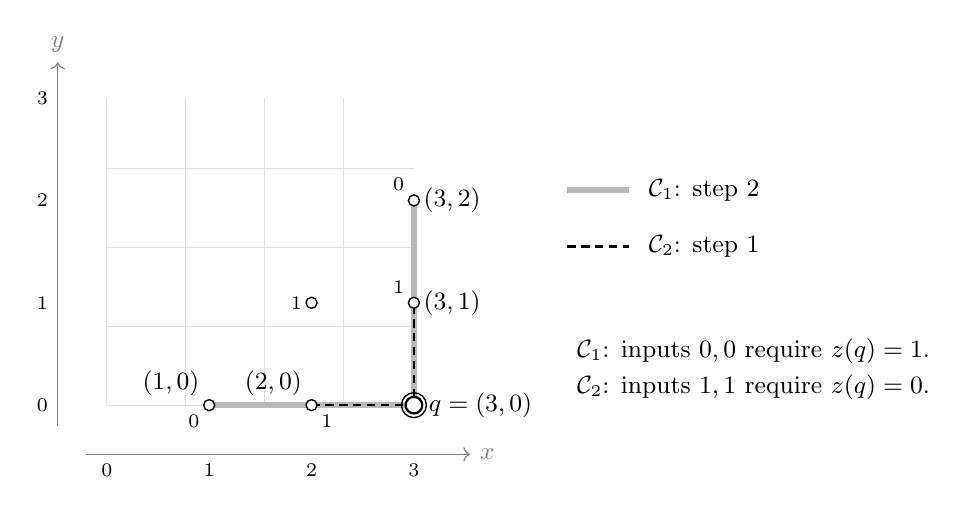
\begin{tikzpicture}[x=13mm,y=13mm,font=\small]
  % Geometric line styles distinguish the corners; they are not cell colors.
  \draw[gray!25,thin] (0,0) grid (3,3);
  \draw[->,gray] (-.2,-.48)--(3.55,-.48) node[right] {$x$};
  \draw[->,gray] (-.48,-.2)--(-.48,3.35) node[above] {$y$};
  \foreach \i in {0,1,2,3}{
    \node[below,font=\scriptsize] at (\i,-.48) {$\i$};
    \node[left,font=\scriptsize] at (-.48,\i) {$\i$};
  }
  \draw[gray!55,line width=2.2pt] (1,0)--(3,0)--(3,2);
  \draw[black,densely dashed,line width=.8pt] (2,0)--(3,0)--(3,1);
  \foreach \p in {(1,0),(2,0),(2,1),(3,1),(3,2)}
    \draw[fill=white,line width=.5pt] \p circle[radius=2pt];
  \draw[fill=white,line width=.8pt] (3,0) circle[radius=3pt];
  \draw[line width=.5pt] (3,0) circle[radius=4.5pt];
  \node[above left] at (1,0) {$(1,0)$};
  \node[above left] at (2,0) {$(2,0)$};
  \node[right] at (3.05,0) {$q=(3,0)$};
  \node[right] at (3,1) {$(3,1)$};
  \node[right] at (3,2) {$(3,2)$};
  \draw[gray!55,line width=2.2pt] (4.5,2.1)--(5.1,2.1);
  \node[anchor=west] at (5.2,2.1) {$\mathcal C_1$: step $2$};
  \draw[black,densely dashed,line width=.8pt] (4.5,1.55)--(5.1,1.55);
  \node[anchor=west] at (5.2,1.55) {$\mathcal C_2$: step $1$};
  \node[anchor=west,align=left,font=\small] at (4.5,.35)
    {$\mathcal C_1$: inputs $0,0$ require $z(q)=1$.\\[2pt]
     $\mathcal C_2$: inputs $1,1$ require $z(q)=0$.};
  \node[below left,font=\scriptsize] at (1,0) {$0$};
  \node[below right,font=\scriptsize] at (2,0) {$1$};
  \node[left,font=\scriptsize] at (2,1) {$1$};
  \node[above left,font=\scriptsize] at (3,1) {$1$};
  \node[above left,font=\scriptsize] at (3,2) {$0$};
\end{tikzpicture}
\caption{\rev{Two directed corners share the completion $(3,0)$.
Line styles distinguish geometric corners, not cell colors.
The five specified cell colors are shown beside the unfilled circles. The shared completion $q$ cannot satisfy both requirements. The circles are the six cells of $V(\{0,1,2,3\})$.}}
\label{fig:shared-completion}
\end{figure}
\FloatBarrier
\end{revision}

For the signed identities, encode the two colors as $-1$ and $1$.
The fiber sum $s_d$ below is then the difference between the two color-class
sizes. The graph uses one vertex for each physical source cell.

\begin{samepage}
\begin{theorem}[Signed completion and physical forcing]\label{thm:forcing}
Let $z:V(A)\to\{-1,1\}$ be proper. For $q=(v,u)\in V(A)$, define
\[
\begin{gathered}
D_q=\{d\in\Z:0<d<v-u,\ u+d,v-d\in A\},\\
p_{q,d}=(u+d,u),\qquad r_{q,d}=(v,v-d),\\
(Kz)_q=\frac12\sum_{d\in D_q}\bigl(z(p_{q,d})+z(r_{q,d})\bigr),\qquad
H_q=\#\{d\in D_q:z(p_{q,d})=z(r_{q,d})\}.
\end{gathered}
\]
Here $K$ is the linear operator specified by this formula and
$\force=\sum_qH_q$. Then
\begin{equation}\label{eq:pointwise-forcing}
H_q=-z(q)(Kz)_q=|(Kz)_q|.
\end{equation}
Insert the two edges $pq$ and $rq$ for each forcing corner with
inputs $p,r$ and completion $q$. The resulting graph $\Gamma$ on $V(A)$
is simple and bipartite under $z$. Writing
$s_d=\sum_{u\in F_d}z(u+d,u)$, it satisfies
\begin{equation}\label{eq:forcing-identity}
|E(\Gamma)|=2\force,\qquad
\force=\frac{2T-M+\sum_ds_d^2}{4},\qquad
2T=M+2|E(\Gamma)|-\sum_ds_d^2.
\end{equation}
If $b(p)$ counts the cells of $p$'s color in its fiber, including $p$,
then $\deg_\Gamma(p)=b(p)-1+2H_p$.
\end{theorem}
\end{samepage}
\begin{proof}
The set $D_q$ indexes exactly the corners completed at $q$.
Their positive step is $v-u-d$, and their two input cells are distinct,
also when $u+d=v-d$.
Opposite input signs contribute zero to $(Kz)_q$.
Equal input signs must both be $-z(q)$ by properness, proving
\eqref{eq:pointwise-forcing}.

The edges $pq$ and $rq$ are horizontal and vertical, respectively.
A horizontal pair $(a,u),(v,u)$ with $a<v$ determines its unique
third cell $(v,u+v-a)$. A vertical pair similarly determines its
third cell. Thus no two corners insert the same edge.
Every inserted edge joins opposite signs, proving simplicity,
bipartiteness, and $|E(\Gamma)|=2\force$.
As an input, $p$ pairs with its $b(p)-1$ other same-color fiber cells.
As an output, it receives two edges for each of its $H_p$ forcing
corners. The two roles give disjoint edges: a completion has
larger coordinate difference than either input. Adding their contributions
proves the degree formula.

The color-class sizes in a fiber are $(r_d+s_d)/2$ and $(r_d-s_d)/2$.
Its equal-sign pairs number
\[
\binom{(r_d+s_d)/2}{2}+\binom{(r_d-s_d)/2}{2}
=\frac{r_d^2+s_d^2-2r_d}{4}.
\]
Every such pair has a unique valid completion by Proposition~\ref{prop:counts}.
Summing and using \eqref{eq:source-counts} proves the remaining
identities in \eqref{eq:forcing-identity}.
\end{proof}

Orient every edge toward its endpoint with larger coordinate difference.
This orientation is acyclic, with outdegree $b(p)-1$ and indegree $2H_p$.
A general corner bound requires control of
$2|E(\Gamma)|-\sum_ds_d^2$ using these geometric restrictions.
Bipartiteness alone is insufficient.

\begin{revision}
G9 is a candidate bound on the number of forcing edges. The coefficient $9$ in~\eqref{eq:forcing-identity} would give $T\le19M/2$ and then $M\le20L$. Neither this edge bound nor its optimality is proved here. A proof could use the geometry beyond bipartiteness: each edge is horizontal or vertical, determines a unique corner, and points toward a larger coordinate difference.
\end{revision}

\begin{assertion}[G9]\label{open:g9}
For every finite $A\subset\Z$ and every proper two-coloring of $V(A)$,
the forcing graph satisfies $|E(\Gamma)|\le9M(A)$.
\end{assertion}

\begin{proposition}[Conditional consequence of G9]\label{prop:g9}
Assume G9. Every properly two-colored strict source satisfies
$T\le19M/2$ and $M\le20L$.
For S21, it suffices that G9 hold for $L\le99\,994$.
\end{proposition}
\begin{proof}
Equation~\eqref{eq:forcing-identity} gives $2T\le M+18M=19M$.
Corollary~\ref{cor:span} then gives $M\le20L$.
The argument holds on any assumed span range. Since $20L\le21L$,
it implies S21 on its stated range.
\end{proof}

Let $\mathcal Z(A)$ be the finite set of proper maps
$z:V(A)\to\{-1,1\}$, and write $\Gamma_z,s_d(z)$ for their graphs
and fiber imbalances. The source bounds require only one
suitable coloring.

\begin{assertion}[Existential G9]\label{open:g9-exists}
\rev{For every finite $A\subset\Z$ with $\mathcal Z(A)\ne\varnothing$, some $z\in\mathcal Z(A)$ satisfies $|E(\Gamma_z)|\le9M(A)$.} Denote this assertion by $\mathrm{G9}^{\exists}$.
\end{assertion}

\begin{proposition}[Consequences of selecting a coloring]\label{prop:g9-exists}
Assume $\mathrm{G9}^{\exists}$. Every strict source admitting a proper
two-coloring satisfies $T\le19M/2$ and $M\le20L$.
For $R_3(\Lconf)\le361$, it suffices to assume
$\mathrm{G9}^{\exists}$ for sources of span at most $360$.
\end{proposition}
\begin{proof}
Choose the coloring supplied by $\mathrm{G9}^{\exists}$ and apply
\eqref{eq:forcing-identity}, followed by Corollary~\ref{cor:span}.
On the restricted span range, Proposition~\ref{prop:span-r3} with
$q=20$ gives the stated Ramsey consequence.
\end{proof}

G9 implies $\mathrm{G9}^{\exists}$, and both assertions remain open.
For any nonempty $\mathcal Z(A)$, \eqref{eq:forcing-identity} also gives
\begin{equation}\label{eq:coloring-selection}
\min_{z\in\mathcal Z(A)}|E(\Gamma_z)|
=T(A)-\frac{M(A)}2
+\frac12\min_{z\in\mathcal Z(A)}\sum_ds_d(z)^2.
\end{equation}
The minima are attained because $\mathcal Z(A)$ is finite.
Minimizing forcing edges therefore amounts to minimizing squared fiber
imbalance. The expression
$2|E(\Gamma_z)|-\sum_ds_d(z)^2=2T(A)-M(A)$ is independent of $z$.
A uniform linear corner bound for general sources remains open.

\section{Six-mark extremizers}\label{sec:six-mark-extremizers}\label{subsec:six-mark-extremizers}
For finite mark sets in $\Z$, we determine the six-mark maximum using an
endpoint deficit, an explicit attaining coloring, and a classification of
the equality sets. The classification concerns the marks and makes no
uniqueness claim for their colorings.

The unrestricted energy bound $E(A)\le n(2n^2+1)/3$, attained by arithmetic
progressions, is classical~\cite[Introduction]{Heg23}. We include a proof before
deriving the nonprogression deficit. We then isolate the endpoint equality
condition, classify the possible five- and six-mark equality sets, and finish
with the proper-coloring certificate.

\begin{lemma}[Endpoint deficit and the six-term obstruction]\label{lem:small}
Every $r$-mark integer set has $T\le\binom r3$ and $E\le e_r=r(2r^2+1)/3$. If $r\ge3$ and the set is not an arithmetic progression, then
\begin{equation}\label{eq:nonprogression-deficit}
T\le\binom r3-(r-2),\qquad E\le e_r-4(r-2).
\end{equation}
Thus equality in the general corner bound forces an arithmetic progression whenever $r\ge2$. A four-mark set whose positive difference multiplicities are at most two has $T\le2$ and $E\le36$. A six-mark nonprogression has $T\le16$ and $E\le130$.
\end{lemma}
\begin{proof}
Order the marks as $a_1<\cdots<a_r$. A difference collision with starts $a_i<a_j$ and larger endpoint $a_k=a_j+d$ gives a triple $i<j<k$. This recovers $d=a_k-a_j$ and the fourth mark $a_i+d$, proving $T\le\binom r3$. The energy identity gives $E\le e_r$, also for $r=0,1$.

We prove the deficit by induction on $r$. Deleting the maximum removes at most $\binom{r-1}{2}$ corners. If all these corners occur, put $h=a_r-a_{r-1}$. For each $i<r-1$, the triple $(i,r-1,r)$ forces $a_i+h$ into the set. The same holds for $a_{r-1}$. Iteration from any mark reaches the maximum, placing every mark in $a_r+h\Z$. Starting at the minimum supplies all intervening terms, so the set is a progression. A nonprogression therefore loses at most $\binom{r-1}{2}-1$ corners on deleting the maximum, and reflection gives the same bound at the minimum.

For $r=3$, this gives $T=0$. For $r\ge4$, some endpoint deletion leaves a nonprogression. Otherwise the two remaining progressions share the consecutive marks $a_2,a_3$, hence have the same step and make the whole set a progression. Choose a deletion leaving a nonprogression and apply induction. Then
\[
T\le\binom{r-1}{3}-(r-3)+\binom{r-1}{2}-1
=\binom r3-(r-2).
\]
The energy identity gives the second inequality in \eqref{eq:nonprogression-deficit}. The equality assertion follows, since every two-mark set is a progression.

For four marks with multiplicities at most two, $2\binom{r_d}{2}\le r_d$ for every positive difference. The unique largest difference makes this inequality strict. Summing gives $2T\le M-1=5$, hence $T\le2$ and $E\le36$.

The six-mark nonprogression bounds follow from \eqref{eq:nonprogression-deficit}. To apply this deficit to properly colored six-mark sources, exclude a six-term progression as follows. Normalize it to $\{0,\ldots,5\}$. Its rows, columns, and offset diagonals each have lengths $1,\ldots,5$. Every pair on any of these lines belongs to exactly one corner. A line of length $j$ has at least $\phi(j)=\binom j2-\lfloor j^2/4\rfloor$ equal-color pairs. Each proper two-colored corner has exactly one equal-color pair, but
\[
3\sum_{j=1}^5\phi(j)=3(0+0+1+2+4)=21>20=T.
\]
This contradiction excludes a six-term progression.
\end{proof}

\subsection{Equality in endpoint deletion}
\begin{lemma}[A single failed pair]\label{lem:endpoint-equality}
Let $X\subset\Z$ be a finite nonprogression with $\min X=0$, put $L=\max X$,
and let $B=X\setminus\{L\}$. The loss at the maximum is
\begin{equation}\label{eq:endpoint-equality-loss}
\begin{split}
\ell_L(X)&:=T(X)-T(B)\\
&=\sum_{\substack{u,v\in B\\u<v}}\ind_{L-v+u\in B}
=\sum_{h>0}r_h(B)\ind_{L-h\in B}.
\end{split}
\end{equation}
It satisfies $\ell_L(X)\le\binom{|B|}{2}-1$, and its deficit counts failed pairs:
\begin{equation}\label{eq:failed-endpoint-pairs}
\binom{|B|}{2}-\ell_L(X)
=\sum_{h>0}r_h(B)\ind_{L-h\notin B}.
\end{equation}
If $\ell_L(X)=\binom{|B|}{2}-1$, precisely one unordered pair fails and
\begin{equation}\label{eq:repeated-difference-extension}
r_h(B)\ge2\quad\Longrightarrow\quad L-h\in B.
\end{equation}
\end{lemma}
\begin{proof}
The removed corner associated with $u<v$ is
$(L-v+u,u),(L,u),(L,v)$, and its first coordinate belongs to $B$ exactly under the displayed membership condition. These parameters recover every removed corner uniquely.

If every pair succeeds, put $b=\max B$ and $h=L-b$. For each $x<b$, the pair $(x,b)$ gives $x+h\in X$, and $b+h=L$. Thus every mark other than $L$ has its translate by $h$ in $X$. Iteration reaches $L$ from every mark, so all marks are congruent modulo $h$. Iteration from zero supplies every intermediate multiple. This would make $X$ a progression. Consequently a nonprogression loses at most
\(\binom{|B|}{2}-1\) corners at this endpoint.

The failed-pair identity follows by subtracting the successful pairs from all
\(\binom{|B|}{2}\) pairs in \(B\). If precisely one pair fails, each difference
represented at least twice must satisfy the membership condition. Otherwise
all its representations would fail, giving at least two failed pairs.
This proves \eqref{eq:repeated-difference-extension}.
\end{proof}

For a nonprogression with at least four marks, the proof of Lemma~\ref{lem:small}
shows that some endpoint deletion leaves a nonprogression. Reflection lets us
take this endpoint to be the maximum. At equality in the deficit bound, both
the surviving set and the endpoint loss must attain their respective bounds.
This equality condition restricts the possible five- and six-mark sets.

\subsection{Classification of the equality sets}
\begin{lemma}[Five-mark equality sets]\label{lem:five-mark-equality}
A five-mark integer set $X$ has $T(X)=7$ exactly when it is a translate and
positive integer dilation of one of
\[
S_0=\{0,1,2,3,5\},\qquad S_1=\{0,2,3,4,5\}.
\]
\end{lemma}
\begin{proof}
We first classify the four-mark sets that can remain after an endpoint deletion.
For four ordered marks with gaps $p,q,s>0$, translate the first mark to zero and write
$Y=\{0,p,p+q,p+q+s\}$. Directly separating four-mark equal-sum patterns from three-term progressions gives
\[
T(Y)=2\ind_{p=s}+\ind_{p=q}+\ind_{q=s}
+\ind_{p=q+s}+\ind_{s=p+q}.
\]
The first condition contributes the two distinct collisions on all four marks. The other four conditions correspond to the four possible three-mark progressions. Thus the complete list of nonprogressions with $T(Y)=2$ consists, after translation, of
\[
\{0,a,b,a+b\}\quad(0<a<b,\ b\ne2a),
\qquad d\{0,1,2,4\},\qquad d\{0,2,3,4\},
\]
with positive integer parameters. To check exhaustiveness, if $p=s$, then $T=2$ requires $q\ne p$, giving the first type. If $p\ne s$, two of the remaining indicators can hold only as $p=q,\ s=2p$ or $q=s,\ p=2q$, giving the last two types.

Now let $|X|=5$ and $T(X)=7$. A five-term progression has $\binom53=10$ corners, so $X$ is not a progression. Choose an endpoint deletion leaving a nonprogression $B$, reflect if necessary so that it deletes the maximum, and translate the minimum to zero. Lemmas~\ref{lem:small} and~\ref{lem:endpoint-equality} give
\[
7=T(B)+\ell_L(X)\le2+5.
\]
Both inequalities are equalities, so the four-mark list applies and every repeated difference satisfies~\eqref{eq:repeated-difference-extension}.

For $B=\{0,a,b,a+b\}$, the differences $a,b$ each occur twice. Since $L>a+b$, the condition $L-a\in B$ forces $L-a=a+b$, hence $L=2a+b$. The condition $L-b\in B$ would then give $2a\in B$, impossible when $0<a<b$ and $b\ne2a$.
For $B=d\{0,1,2,4\}$, the repeated differences $d,2d$ force $L=5d$ and then $L-2d=3d\in B$, again impossible.
For $B=d\{0,2,3,4\}$, they force $L=5d$. This extension does have five successful pairs: the differences $d,2d,3d$ succeed, and only the single pair at difference $4d$ fails. Undoing the optional reflection gives the two stated forms.
Conversely, both have multiplicities $(3,3,2,1,1)$ at their five positive differences and hence $T=7$.

\end{proof}

\begin{proposition}[Six-mark equality sets]\label{prop:six-mark-classification}
Put $A_*=\{0,1,2,3,4,6\}$. A six-mark integer set $A$ has $T(A)=16$
exactly when
\begin{equation}\label{eq:six-point-equality-classification}
A=a+dA_*\quad\hbox{or}\quad A=a+d(6-A_*),
\qquad a\in\Z,\ d\in\Z_{>0},
\end{equation}
where $6-A_*=\{0,2,3,4,5,6\}$.
\end{proposition}
\begin{proof}
Let $|A|=6$ and $T(A)=16$. A six-term progression has $\binom63=20$ corners, so $A$ is not a progression. Select a nonprogression endpoint deletion, reflect so that the endpoint is the maximum $L$, and translate the minimum to zero. The same equality argument gives
\[
16=T(B)+\ell_L(A)\le7+9,
\]
so $B=dS_0$ or $dS_1$, and every repeated difference must succeed. For either type the differences $d,2d,3d$ have multiplicities $3,3,2$, respectively. Since $L>5d$, the condition $L-d\in B$ forces $L=6d$. The type $dS_0$ is impossible because $L-2d=4d\notin dS_0$. The type $dS_1$ gives precisely one failed pair, at difference $5d$, while its other differences succeed. Therefore the normalized six-mark set is
$d\{0,2,3,4,5,6\}=d(6-A_*)$. Undoing translation and the possible reflection proves~\eqref{eq:six-point-equality-classification}. 


Conversely, the positive-difference multiplicities of $A_*$ are
$(4,4,3,2,1,1)$ at differences $1,\ldots,6$. Hence $T(A_*)=16$ by
Proposition~\ref{prop:counts}. Translation, positive dilation and reflection
preserve equality of differences, so both forms in
\eqref{eq:six-point-equality-classification} have the same corner count.
\end{proof}

\subsection{The maximum under proper two-coloring}
\begin{corollary}[The exact six-mark maximum]\label{prop:six-point-extremal}
Among six-mark integer sets $A$ whose strict sources admit proper two-colorings, the maximum values of $T(A)$ and $E(A)$ are respectively $16$ and $130$. Both are attained by
\[
A_*=\{0,1,2,3,4,6\}.
\]

Equality in either maximum holds exactly for the sets in
\eqref{eq:six-point-equality-classification}. The maximizer has one type up to
translation, positive integer dilation and reflection.
\end{corollary}
\begin{proof}
Lemma~\ref{lem:small} excludes a proper two-coloring for a six-term progression and gives $T\le16$ for every other six-mark set. Hence every source in the stated class has $T\le16$, and Proposition~\ref{prop:counts} gives $E\le2\cdot6^2-6+4\cdot16=130$.

For attainment, the left-hand part of Table~\ref{tab:six-point-witness} defines a coloring $z:V(A_*)\to\{0,1\}$. Row $v$ reads the colors of $(v,u)$ in increasing order of $u\in A_*$ with $u<v$, so all fifteen cells are specified. For a corner of common leg length $h$, read its color word in the order
\[
(x,y),\quad (x+h,y),\quad (x+h,y+h).
\]
The positive-difference multiplicities at $d=1,\ldots,6$ are $(4,4,3,2,1,1)$, so Proposition~\ref{prop:counts} gives $T(A_*)=6+6+3+1=16$. The right-hand part lists these sixteen corner words in lexicographic order of the admissible bases $(x,y)$ for each $h$. Only $1\le h\le6$ is possible, and every word uses both colors. Thus the coloring is proper, and the energy identity gives $E(A_*)=130$.

\begin{table}[H]
\centering
\ifshowrevisions\color{red}\fi
\caption{\rev{A complete six-mark coloring and all its corner color words. The left table specifies the rows of $V(A_*)$. The right table lists every corner by common leg length.}}
\label{tab:six-point-witness}
\begin{tabular}{@{}rl@{}}
\toprule
$v$ & Row word\\\midrule
1 & \texttt{1}\\
2 & \texttt{01}\\
3 & \texttt{100}\\
4 & \texttt{0010}\\
6 & \texttt{11000}\\
\bottomrule
\end{tabular}
\qquad
\begin{tabular}{@{}rrl@{}}
\toprule
$h$ & Count & Corner color words\\\midrule
1 & 6 & \texttt{101}, \texttt{010}, \texttt{100}, \texttt{100}, \texttt{001}, \texttt{010}\\
2 & 6 & \texttt{110}, \texttt{001}, \texttt{100}, \texttt{010}, \texttt{010}, \texttt{100}\\
3 & 3 & \texttt{100}, \texttt{110}, \texttt{010}\\
4 & 1 & \texttt{010}\\
5,6 & 0 & ---\\
\bottomrule
\end{tabular}
\end{table}

Proposition~\ref{prop:six-mark-classification} gives all possible mark sets
at $T=16$. The energy identity makes equality at $E=130$ equivalent to
equality at $T=16$.

Finally, both forms in~\eqref{eq:six-point-equality-classification} inherit a proper coloring from the displayed witness. Translation and positive dilation act on cells by $(x,y)\mapsto(a+dx,a+dy)$ and preserve positive directed L's. A reflected mark map $t\mapsto c-dt$ acts on strict cells by
\[
(x,y)\longmapsto(c-dy,c-dx).
\]
For a corner $(p,q,r)$ in input--completion--input order, its three images in reverse order form a positive directed L of step $d$ times the original step. Reflection therefore preserves properness, so every equality set inherits a proper coloring.

\end{proof}

\section{Structured sources}\label{sec:structured}
Table~\ref{tab:structured} lists the linear corner bounds proved in this
section. For complete products, energy factors into the energies of the
factors. Translation matchings are controlled by difference correlations.
In two-distance representations, additive relations become squares. Throughout, $n=|A|$, $M=\binom n2$, and $L=L(A)$.

\subsection{Complete products}
\begin{table}[H]
\centering
\caption{Leading corner and span bounds for proper two-colorings. The theorems state all hypotheses and any stronger linear terms. The strict matching span bound assumes $A\ne\varnothing$.}
\label{tab:structured}
\begin{tabular}{@{}lccc@{}}
\toprule Family & Reference & Corner bound & Span bound\\\midrule
Complete progression products & Theorem~\ref{thm:progression} & $T\le7M/2$ & $M\le8L$\\
Complete direct sums & Theorem~\ref{thm:direct} & $T\le23M/4$ & $M\le25L/2$\\
Translation matchings & Theorem~\ref{thm:matching} & $T\le10M$ & $M<18L$\\
Two-distance representations & Theorem~\ref{thm:two_distance} & $T\le6M$ & $M\le13L$\\
At most three long pairs per midpoint & Theorem~\ref{thm:midpoint-three} & $T\le2M$ & $M\le5L$\\
\bottomrule
\end{tabular}
\end{table}
\begin{theorem}[Complete progression products]\label{thm:progression}
Let $B\subset\Z$ be finite and nonempty, let $t\ge2$ and $Q>2L(B)$ be integers, and put $A=B+Q\{0,\ldots,t-1\}$ and $n=t|B|$. If $V(A)$ admits a proper two-coloring, then
\begin{equation}\label{eq:progression-bounds}
E(A)\le9n^2-15n,\qquad
T(A)\le\frac72M-\frac74n,\qquad M\le8L.
\end{equation}
These conclusions also follow from the weaker assumption that $B+Q\{0,\ldots,t-2\}$ is a union of two disjoint Golomb sets.
\end{theorem}
\begin{proof}
Write $b=|B|$ and $P_s=\{0,\ldots,s-1\}$. Separation $Q>2L(B)$ gives unique mark representations and $F_Q=B+QP_{t-1}$. By Lemmas~\ref{lem:restriction} and~\ref{lem:golomb}, this fiber is a union of two Golomb classes. Theorem~\ref{thm:energy} therefore gives $E(F_Q)\le6(t-1)^2b^2-5(t-1)b$. The weaker assumption gives the same estimate directly.

An equality of differences in $B+QP_s$ has base discrepancy of magnitude at most $2L(B)<Q$. The base and layer differences therefore agree separately, giving
\begin{equation}\label{eq:product-energy}
E(B+QP_s)=E(B)e_s,\qquad
e_s=E(P_s)=s^2+2\sum_{j=1}^{s-1}(s-j)^2=\frac{s(2s^2+1)}3.
\end{equation}
Put $D_t=2(t-1)^2+1$, $R_t=(2t^2+1)/D_t$, and $\lambda_t=6(t-1)R_t/t$. Taking the ratio in \eqref{eq:product-energy} gives
\begin{equation}\label{eq:progression-comparison}
E(A)\le\lambda_t n^2-5R_tn,\qquad
9-\lambda_t=\frac{3(t-2)(2t^2-4t-1)}{tD_t}\ge0.
\end{equation}
For $t=2$, the first bound is exactly $9n^2-15n$. For $t=3,4$, the quantity $(9-\lambda_t)n+5R_t-15$ is respectively $(15b-40)/9$ and $(90b-120)/19$, so it is nonnegative when $b\ge3$ and $b\ge2$. For $t\ge5$, use $n\ge t$ to bound it below by
\[
\frac{6t^3-44t^2+81t-34}{D_t}
=\frac{6(t-5)^3+46(t-5)^2+91(t-5)+21}{D_t}>0.
\]
The remaining pairs $(t,b)=(3,1),(3,2),(4,1)$ have energies $19,114,44$ by \eqref{eq:product-energy}, below the respective target values $36,234,84$. Thus $E(A)\le9n^2-15n$ in every case. Proposition~\ref{prop:counts} gives the corner bound, and its weaker consequence $T\le7M/2$ gives $M\le8L$ by Corollary~\ref{cor:span}.
\end{proof}

\begin{theorem}[Complete direct sums]\label{thm:direct}
Let $B,C\subset\Z$ be finite with $b=|B|\ge2$ and $c=|C|\ge2$, and let $Q>2L(B)$ be an integer. If the complete sum $A=B+QC$ admits a proper two-coloring of $V(A)$, then, with $n=bc$,
\begin{equation}\label{eq:direct-bounds}
E(A)\le\frac{27n^2-25n}{2},\qquad T(A)\le\frac{23}{4}M,\qquad M\le\frac{25}{2}L.
\end{equation}
\end{theorem}
A monochromatic rectangle in a fiber would repeat a difference within one Golomb class. This obstruction restricts both factors.

\begin{lemma}[Complete overlap restrictions]\label{lem:rectangles}
Under the hypotheses of Theorem~\ref{thm:direct}, $E(A)=E(B)E(C)$ and each factor is a union of two Golomb sets. If one factor has at least seven marks, every positive difference multiplicity of the other is at most two. If one has at least five marks, those multiplicities are at most four.
\end{lemma}
\begin{proof}
Separation gives the energy product as in \eqref{eq:product-energy}. It also gives
\begin{equation}\label{eq:product-fibers}
\begin{aligned}
F_h&=(B\cap(B-h))+QC &&\text{for }h\in\Delta B,\\
F_{Q\delta}&=B+Q(C\cap(C-\delta)) &&\text{for }\delta\in\Delta C.
\end{aligned}
\end{equation}
Lemma~\ref{lem:golomb} partitions each fiber into two Golomb classes. Fixing a base mark in the first fiber gives a translate of $QC$. Fixing a layer in the second gives a translate of $B$. Both factors therefore have two-Golomb partitions.

Neither fiber array can contain a monochromatic rectangle, which would repeat a nonzero difference in one class. Every two-colored $7\times3$ array has such a rectangle: each row contains a same-color pair, and there are only $2\binom32=6$ choices of pair and color. A $5\times5$ array also has one. Otherwise each row-pair/color label occurs in at most one column, allowing at most $2\binom52=20$ same-color row pairs. Each column contributes at least four, forcing all columns to split $2+3$ and each color to use all ten row pairs. If $k$ columns have three red entries, the red-pair count is $5+2k\ne10$, a contradiction. Apply these two rectangle obstructions to \eqref{eq:product-fibers}, transposing the arrays when necessary.
\end{proof}

\rev{Fixing a layer or a base mark embeds either factor's strict source into $V(A)$. Hence a six-mark factor admits a proper source coloring, and Corollary~\ref{prop:six-point-extremal} gives its energy bound $130$.}

\begin{proof}[Proof of Theorem~\ref{thm:direct}]
By Lemma~\ref{lem:rectangles} and Theorem~\ref{thm:energy}, the factor energies are at most $6b^2-5b$ and $6c^2-5c$. By symmetry, assume $b\le c$.

For $2\le r\le5$, $e_r/r^2=(2r+r^{-1})/3\le17/5$. If $c\le5$ and $n\ge8$, then
\[
\frac{E(A)}{n^2}\le\frac{289}{25}<\frac{191}{16}
\le\frac{27}{2}-\frac{25}{2n}.
\]
The remaining sizes $n=4,6$ have energies at most $36,114$, which satisfy the same bound. If $c=6$ and $b\le5$, Lemma~\ref{lem:small} gives
\[
\frac{E(A)}{n^2}\le\frac{17}{5}\frac{130}{36}
=\frac{221}{18}<\frac{299}{24}
\le\frac{27}{2}-\frac{25}{2n},
\]
since $n\ge12$. If $b=c=6$, then $E(A)\le130^2=16\,900<17\,046=(27\cdot36^2-25\cdot36)/2$.

Suppose now that $c\ge7$. A positive difference multiplicity cap $k$ gives
\begin{equation}\label{eq:multiplicity-energy}
E(S)=|S|^2+2\sum_{h>0}r_S(h)^2
\le(k+1)|S|^2-k|S|.
\end{equation}
Lemma~\ref{lem:rectangles} gives cap two on $B$. If $b=2,3,4$, Lemma~\ref{lem:small} bounds $E(B)$ by $6,19,36$, respectively. Multiplying by $E(C)\le6c^2-5c$ yields
\[
E(A)\le
\begin{cases}
9n^2-15n,&b=2,\\
(38n^2-95n)/3,&b=3,\\
27n^2/2-45n,&b=4.
\end{cases}
\]
Each is at most $(27n^2-25n)/2$. For $b=5,6$, the cap four on $C$ gives
\[
E(A)\le(15-10/b)n^2-(12b-8)n
\le\tfrac{40}{3}n^2-52n<\tfrac{27n^2-25n}{2}.
\]
If $b\ge7$, both factors have cap two, so $E(A)\le9n^2<(27n^2-25n)/2$ because $n\ge49$. The energy bound is proved. Proposition~\ref{prop:counts} and Corollary~\ref{cor:span} yield the corner and span bounds.
\end{proof}
The optimal constants for complete products remain open. The proofs require every factor pair to be present. Filling missing pairs can destroy properness, so the bounds do not extend by completion to partial products.

\subsection{Translation matchings}
\begin{theorem}[Translation matchings]\label{thm:matching}
Let $S\subset\Z$ be finite and $d>0$ an integer. Suppose $A=S\sqcup(S+d)$ admits a proper two-coloring of $V(A)$. With $n=2|S|$,
\begin{equation}\label{eq:matching-energy}
E(A)\le22n^2-41n,\qquad T(A)\le10M-5n.
\end{equation}
If $S\ne\varnothing$, then $L\ge1$ and
\begin{equation}\label{eq:matching-span}
M\le16L-13+3\sqrt{8L-7}<18L.
\end{equation}
The translates and their difference ranges need not be separated. For $S=\varnothing$, only \eqref{eq:matching-energy} is asserted.
\end{theorem}
\begin{proof}
Partition $S=B\sqcup C$ by the colors of $(x+d,x)$. Since $S\subseteq F_d$, Lemma~\ref{lem:golomb} makes both classes Golomb. The four sets $B,C,B+d,C+d$ are pairwise disjoint.

For a nonempty Golomb set $B$ of size $b$, let $r_B(t)$ count ordered representations of the signed difference $t$, and put $C_h(B)=\sum_t r_B(t)r_B(t+h)$ for $h>0$. Here $r_B(0)=b$, each nonzero multiplicity is at most one, and $E(B)=2b^2-b$. If $r_B(h)=0$, then $C_h(B)\le b(b-1)$. If $r_B(h)=1$, the terms at $t=0,-h$ contribute $2b$. Among nonzero differences, $-h$ has already been counted and the largest positive difference contributes zero. Hence $C_h(B)\le b^2+b-2$, which also bounds the first case for $b\ge1$.

For $P_B=B\sqcup(B+d)$, expansion of the four translate types gives
\begin{equation}\label{eq:matching-correlation}
\begin{aligned}
r_{P_B}(t)&=2r_B(t)+r_B(t-d)+r_B(t+d),\\
E(P_B)&=6E(B)+8C_d(B)+2C_{2d}(B).
\end{aligned}
\end{equation}
Disjointness gives $r_B(d)=0$. Thus
\begin{equation}\label{eq:matching-class}
E(P_B)\le6(2b^2-b)+8(b^2-b)+2(b^2+b-2)
=g(b),\qquad g(t)=22t^2-12t-4.
\end{equation}

To bound the energy of a union, take disjoint finite $X,Y$ and let $q_{X,Y}(t)$ count pairs with $y-x=t$. Count solutions of $y-x=y'-x'$ by the common difference $x'-x=y'-y$ and apply Cauchy--Schwarz:
\[
\sum_t q_{X,Y}(t)^2=\sum_t r_X(t)r_Y(t)\le\sqrt{E(X)E(Y)}.
\]
Since $r_{X\sqcup Y}=r_X+r_Y+q_{X,Y}+q_{Y,X}$, the Euclidean triangle inequality yields
\begin{equation}\label{eq:energy-triangle}
E(X\sqcup Y)^{1/4}\le E(X)^{1/4}+E(Y)^{1/4}.
\end{equation}
Squaring this inequality gives the equivalent bound
$E(X\sqcup Y)^{1/2}\le E(X)^{1/2}+E(Y)^{1/2}+2(E(X)E(Y))^{1/4}$.

For $t\ge1$, $g(t)>0$ and $g^{1/4}$ is concave, because the sign of its second derivative is the sign of
$4gg''-3(g')^2=-1936(t-3/11)^2-992<0$.
If $b,c\ge1$, \eqref{eq:energy-triangle} and concavity give
\[
E(A)\le\bigl[g(b)^{1/4}+g(c)^{1/4}\bigr]^4
\le16g(n/4)=22n^2-48n-64\le22n^2-41n.
\]
If exactly one class is nonempty, \eqref{eq:matching-class} gives $E(A)\le g(n/2)$. Subtracting this bound from $22n^2-41n$ gives $(n-2)(33n/2-2)\ge0$, since $n$ is even and at least two. The empty case is immediate. Proposition~\ref{prop:counts} proves the corner bound.

For nonempty $S$, its span is $L-d\le L-1$. The distinct positive differences in each Golomb class therefore give $\binom b2,\binom c2\le L-1$. Consequently $s=b+c\le1+\sqrt{8L-7}$, and the increasing function $s(2s-1)$ gives the first bound in \eqref{eq:matching-span}. Finally,
\[
(2L+13)^2-9(8L-7)=4(L-5/2)^2+207>0
\]
proves its strict comparison with $18L$. The radical is used only for $L\ge1$.
\end{proof}

\subsection{Two-distance representations}
We use an injective Freiman homomorphism of order two, a map preserving pair-sum equalities~\cite{TV06}. If its squared distances are $\tau$ and $2\tau$, every nontrivial parallelogram in the image is a square. No common sphere is assumed.

\begin{revision}
The two allowed distances force the sides of any nontrivial parallelogram
to be short and its diagonals long. They also exclude three-term
progressions, as the proof below shows.

To count these squares, choose two of the $k_{\mathbf c}$ long pairs at a common midpoint. Each integer four-mark relation contributes two corners, so twice the number of image squares bounds the corner count:
\[
T(A)\le2\sum_{\mathbf c}\binom{k_{\mathbf c}}2
=\sum_{\mathbf c}k_{\mathbf c}(k_{\mathbf c}-1).
\]
The image may have additional pair-sum relations, so this is an inequality. If every $k_{\mathbf c}\le3$, each long pair shares its midpoint with at most two others, giving the coefficient two in Theorem~\ref{thm:midpoint-three}. The family in Corollary~\ref{prop:weight-two-family} has ratio tending to two, proving asymptotic sharpness.
\end{revision}

\begin{theorem}[Two-distance representations]\label{thm:two_distance}
Let $A\subset\Z$ be finite. Suppose an injective map $\phi:A\to\R^r$ and a number $\tau>0$ satisfy
\begin{equation}\label{eq:two-distance-hypotheses}
\begin{gathered}
a+b=c+e\ \Longrightarrow\ \phi(a)+\phi(b)=\phi(c)+\phi(e)
\quad\text{for all }a,b,c,e\in A,\\
\|\phi(a)-\phi(b)\|^2\in\{\tau,2\tau\}\quad\text{for }a\ne b.
\end{gathered}
\end{equation}
Pair-sum preservation includes repeated marks. Then the squared-distance coloring of $V(A)$ is proper, and
\begin{equation}\label{eq:two-distance-bounds}
T(A)\le6M,\qquad M\le13L.
\end{equation}
Preservation is required only in the stated direction.
\end{theorem}
\begin{proof}
\rev{We count squares by their midpoints and remove blocks that share no square with the remaining points. A polynomial argument bounds the remaining set in the eight-pair case, after which a short-pair incidence count completes the estimate. We then transfer the bound to the integer source.}

\medskip\noindent\rev{\emph{Square relations and midpoint counts.}}
Put $X=\phi(A)$. It contains no three-term progression, since its outer squared distance would be four times a side squared distance. Thus every nontrivial equality of unordered pair sums uses four distinct points. If $\mathbf u,\mathbf v$ are adjacent sides of the resulting parallelogram, then
\[
\|\mathbf u+\mathbf v\|^2+\|\mathbf u-\mathbf v\|^2
=2\bigl(\|\mathbf u\|^2+\|\mathbf v\|^2\bigr).
\]
The left side is at most $4\tau$ and the right side at least $4\tau$. Equality forces side squares $\tau$, diagonal squares $2\tau$, and $\langle\mathbf u,\mathbf v\rangle=0$.

Call a pair long when its squared distance is $2\tau$, and let $k_{\mathbf c}$ be the number of long unordered pairs with midpoint $\mathbf c$. Distinct pairs at one midpoint have disjoint endpoints and form a square. Thus twice the number of squares is
\begin{equation}\label{eq:geometric-corners}
T_{\mathrm{geom}}(X)=\sum_{\mathbf c}k_{\mathbf c}(k_{\mathbf c}-1).
\end{equation}
Only finitely many midpoints contribute.

\medskip\noindent\rev{\emph{Large midpoint blocks.}}
Suppose $k=k_{\mathbf c}\ge8$, and let $Y=\{\mathbf c\pm\mathbf p_i:1\le i\le k\}$ contain all endpoints of the long pairs at $\mathbf c$. Each radius has squared norm $\tau/2$. For $i\ne j$, the distances $\|\mathbf p_i\pm\mathbf p_j\|^2$ are at least $\tau$ and sum to $2\tau$, so the radii are orthogonal.

For an outside point $\mathbf c+\mathbf q$, put $t=\|\mathbf q\|^2+\tau/2$. Its squared distances to the endpoints of pair $i$ are $t\mp2\langle\mathbf q,\mathbf p_i\rangle\in\{\tau,2\tau\}$, so $t\in\{\tau,3\tau/2,2\tau\}$. The middle value would give $\|\mathbf q\|^2=\tau$ and $|\langle\mathbf q,\mathbf p_i\rangle|=\tau/4$. Orthogonal projection would then imply
\[
\tau=\|\mathbf q\|^2\ge\sum_i
\frac{\langle\mathbf q,\mathbf p_i\rangle^2}{\|\mathbf p_i\|^2}
=\frac{k\tau}{8}.
\]
For $k\ge9$, the middle value is therefore impossible, so every outside point is orthogonal to the radii after translation by $-\mathbf c$. For $k=8$, equality in the projection bound forces each point in the middle case to have the form $\mathbf q=\tfrac12\sum_{i=1}^8\varepsilon_i\mathbf p_i$, with $\varepsilon_i\in\{-1,1\}$.

If every outside point is orthogonal to the radii, no square meets both $Y$ and its complement. Translate $\mathbf c$ to zero and project the diagonal sums onto the span of the radii. A long pair within $Y$ is antipodal and has projection zero, as does a pair outside $Y$. A pair meeting both sets has projection $\pm\mathbf p_i$, which identifies its endpoint in $Y$. A pair with the same sum must then share the other endpoint too, so it cannot be a distinct diagonal. The remaining possibility is an antipodal pair in $Y$ and an outside long pair of midpoint $\mathbf c$, excluded by the definition of $Y$. Thus
\begin{equation}\label{eq:geometric-removal}
T_{\mathrm{geom}}(X)=k(k-1)+T_{\mathrm{geom}}(X\setminus Y).
\end{equation}
\begin{revision}
\noindent\emph{Deletion of isolated blocks.} Perform the following deletion on the current remaining point set. If a midpoint has $k\ge8$ long pairs and every point outside their $2k$ endpoints is orthogonal to the radii after translation to that midpoint, remove all $2k$ endpoints. Recompute the midpoint multiplicities and test the same condition in the remaining set. Equation~\eqref{eq:geometric-removal} applies at every step, since the two-distance hypotheses are inherited by subsets. Each step removes points, so this process terminates at a set $X_0$ with no eligible midpoint. The projection argument makes every midpoint with $k\ge9$ eligible for deletion. Thus $X_0$ has at most eight long pairs per midpoint. If all multiplicities are at most seven, then $T_{\mathrm{geom}}(X_0)\le6\binom{|X_0|}{2}$.
\end{revision}

\begin{revision}
\noindent\emph{The critical eight-pair case.} Otherwise choose a midpoint of multiplicity eight in $X_0$, translate it to the origin, and write $Y=\{\pm\mathbf p_i:1\le i\le8\}$ for the corresponding endpoints. Since the deletion process has terminated, at least one point $\mathbf q\in X_0\setminus Y$ is not orthogonal to the radii. Fix such a point. The equality case of the projection argument gives $\|\mathbf q\|^2=\tau$ and $\mathbf q=\tfrac12\sum_{i=1}^8\varepsilon_i\mathbf p_i$, so $\mathbf q$ lies in the span of the radii. If another outside point $\mathbf q'$ were orthogonal to that span, the earlier distance calculation would give $\|\mathbf q'\|^2\in\{\tau/2,3\tau/2\}$. It would follow that $\|\mathbf q-\mathbf q'\|^2\in\{3\tau/2,5\tau/2\}$, contrary to the two-distance hypothesis. Thus every outside point is nonorthogonal and has the sign-vector form above. Their sign vectors form a code $\mathcal C\subset\{-1,1\}^8$ with pairwise Hamming distance two or four.
\end{revision} For each $\varepsilon\in\mathcal C$, the polynomial
\[
f_{\varepsilon}(x)=\langle\varepsilon,x\rangle\bigl(\langle\varepsilon,x\rangle-4\bigr)
\]
is $32$ at $\varepsilon$ and zero at every other codeword. These functions are linearly independent on $\mathcal C$. Reducing $x_i^2=1$ puts them in the space spanned by $1$, the eight coordinates, and their $28$ pairwise products. Thus $|\mathcal C|\le37$ and $|X_0|\le53$.

\begin{revision}
\noindent\emph{The final incidence count.} Write $q_8$ for the number of midpoints with eight long pairs, and let $s$ and $\ell$ count the short and long unordered pairs of $X_0$. The sixteen endpoints at each such midpoint have eight antipodal long pairs. Their other $\binom{16}{2}-8=112$ pairs are short. To bound repeated incidences, fix a short pair $\{\mathbf x,\mathbf y\}$ and choose the same endpoint $\mathbf x$ for every midpoint under consideration. If this pair belongs to the endpoint block at $\mathbf c$, then the antipode $\mathbf x_{\mathbf c}=2\mathbf c-\mathbf x$ belongs to $X_0\setminus\{\mathbf x,\mathbf y\}$. Indeed, antipodal pairs are distinct and long, whereas $\{\mathbf x,\mathbf y\}$ is short. The map $\mathbf c\mapsto\mathbf x_{\mathbf c}$ is injective because $\mathbf c=(\mathbf x+\mathbf x_{\mathbf c})/2$. Hence this short pair belongs to at most $|X_0|-2\le51$ endpoint blocks. Counting incidences between blocks and their short pairs gives $112q_8\le51s$.
Every long pair has exactly one midpoint, so $\sum_{\mathbf c}k_{\mathbf c}=\ell$.
For $k_{\mathbf c}\le7$, the contribution is at most $6k_{\mathbf c}$. A midpoint
with eight pairs contributes eight more than this bound. Equivalently,
\[
k_{\mathbf c}(k_{\mathbf c}-1)
\le6k_{\mathbf c}+8\ind_{k_{\mathbf c}=8}.
\]
Summing over midpoints and applying the incidence bound gives
\end{revision}
\begin{equation}\label{eq:two-distance-eight}
T_{\mathrm{geom}}(X_0)\le6\ell+8q_8
\le6\ell+\frac{51}{14}s\le6\binom{|X_0|}{2}.
\end{equation}
Each removed $2k$-point set contributes $k(k-1)\le6\binom{2k}{2}$. The removed blocks and $X_0$ are disjoint, so their internal pairs form a subset of all pairs in the whole set. Summing the block estimates therefore gives $T_{\mathrm{geom}}(X)\le6\binom{|X|}{2}$.

\medskip\noindent\rev{\emph{Return to the integer source.}}
Let $D(A)$ count patterns $a<b<c<e$ with $a+e=b+c$, and let $P_3(A)$ count three-term progressions with distinct marks. A four-mark pattern gives exactly two difference collisions, $b-a=e-c$ and $c-a=e-b$. A progression gives one. Hence
\begin{equation}\label{eq:four-mark-corners}
T(A)=2D(A)+P_3(A).
\end{equation}
Preservation of repeated-mark equalities gives $P_3(A)=0$, and injectivity sends different four-mark patterns to different squares. Therefore $T(A)\le T_{\mathrm{geom}}(X)\le6M$. In each collision, the parallel endpoint cells represent square sides and the outer completion represents a diagonal. Their squared-distance colors are $\tau,\tau,2\tau$, so the coloring is proper. Corollary~\ref{cor:span} gives the span bound.
\end{proof}

\begin{theorem}[Midpoint multiplicity at most three]\label{thm:midpoint-three}
Under \eqref{eq:two-distance-hypotheses}, suppose each midpoint belongs to at most three long unordered pairs in $\phi(A)$. Then
\begin{equation}\label{eq:midpoint-three-bounds}
T(A)\le2M,\qquad M\le5L.
\end{equation}
The squared-distance coloring is proper, and the corner coefficient two is asymptotically optimal within this subclass.
\end{theorem}
\begin{proof}
The preceding proof gives $T(A)\le\sum_{\mathbf c}k_{\mathbf c}(k_{\mathbf c}-1)$. Since $k_{\mathbf c}\le3$, the sum is at most $2\sum_{\mathbf c}k_{\mathbf c}\le2M$, because every long pair has a unique midpoint. Corollary~\ref{cor:span} gives $M\le5L$. Properness follows from Theorem~\ref{thm:two_distance}, and the family in Corollary~\ref{prop:weight-two-family} proves asymptotic optimality.
\end{proof}
The best corner coefficient under the unrestricted two-distance hypotheses remains between two and six. These hypotheses exclude three-term progressions, even though a three-mark progression has a proper strict two-coloring.

\subsection{Sources encoded by graphs}
The simplex-edge configuration $\{e_i+e_j:i<j\}$ is standard in two-distance geometry~\cite{Musin09,BSS12}. Selecting its points by graph edges gives an exact corner count for the corresponding integer source.

\begin{theorem}[Sources encoded by graph edges]\label{thm:graph-source}
Let $G$ be a finite simple graph on $\{0,\ldots,r-1\}$, with $r\ge1$, and let $e_0,\ldots,e_{r-1}$ be the standard basis of $\R^r$. Set
\begin{equation}\label{eq:graph-source}
A_G=\{5^i+5^j:\{i,j\}\in E(G)\},\qquad m=|E(G)|.
\end{equation}
Let $C_4(G)$ count simple four-cycles up to cyclic rotation and reversal, allowing chords. Then $|A_G|=m$, and the map $\phi(5^i+5^j)=e_i+e_j\in\R^r$ preserves pair-sum equalities in both directions, including repeated marks. It satisfies Theorem~\ref{thm:midpoint-three} with $\tau=2$, so its squared-distance coloring is proper. Moreover,
\begin{equation}\label{eq:graph-counts}
\begin{gathered}
T(A_G)=2C_4(G),\qquad E(A_G)=2m^2-m+8C_4(G),\\
T(A_G)\le2\binom m2,\qquad M(A_G)\le5L(A_G).
\end{gathered}
\end{equation}
\end{theorem}
\begin{proof}
Base-five digits determine each edge uniquely. A relation between four marks gives $\sum_i\alpha_i5^i=0$ with $\alpha_i\in\{-2,-1,0,1,2\}$. If $k$ is the largest nonzero index, its term has magnitude at least $5^k$, whereas the smaller terms have total magnitude at most $2\sum_{i<k}5^i=(5^k-1)/2$. Thus all coefficients vanish. This proves equivalence with the vector pair-sum equality, including repeated marks.

Distinct edges have squared image distance two when they meet and four when disjoint. A long pair consists of two disjoint edges on a four-element vertex set $S$, and its midpoint is half the indicator vector of $S$. The long pairs at that midpoint are precisely the available perfect matchings of $G[S]$. Write $k_S$ for their number. The three possible perfect matchings give $k_S\le3$, proving the representation hypotheses and both inequalities.

A pair-sum records the degrees of its two graph edges. A doubled edge and a pair of edges meeting at one vertex each have a unique unordered representation. The only collisions therefore occur between two different perfect matchings of one $S$. No doubled mark shares a sum with another pair, so $P_3(A_G)=0$. Two distinct perfect matchings on $S$ have a four-cycle as their union, and each four-cycle has exactly these two alternating matchings. Hence
\[
D(A_G)=\sum_{|S|=4}\binom{k_S}{2}=C_4(G).
\]
Equation~\eqref{eq:four-mark-corners} proves the corner identity, and Proposition~\ref{prop:counts} gives the energy identity. The collision sums are empty for graphs with no edges or one edge, so the formulas include both cases.
\end{proof}

\begin{revision}
\noindent\textbf{A worked four-vertex graph.}
For $G=K_4$ on $\{0,1,2,3\}$, the six edges give
\begin{equation}\label{eq:k4-worked-set}
A_{K_4}=\{6,26,30,126,130,150\}.
\end{equation}
The three perfect matchings in Table~\ref{tab:k4-worked} have the same sum, so their images share the midpoint $(1,1,1,1)/2$. Any two distinct matchings alternate around a four-cycle, whose alternating edges recover the matchings uniquely. Chords do not merge these cycles. The three pairs of matchings therefore give three unoriented four-cycles and six source corners.

\begin{table}[H]
\centering
\ifshowrevisions\color{red}\fi
\caption{\rev{The three perfect matchings of $K_4$ and their encoded pair sums.}}
\label{tab:k4-worked}
\begin{tabular}{@{}clcc@{}}
\toprule
Matching & Graph edges & Encoded pair & Sum\\\midrule
1 & $\{0,1\},\{2,3\}$ & $6+150$ & 156\\
2 & $\{0,2\},\{1,3\}$ & $26+130$ & 156\\
3 & $\{0,3\},\{1,2\}$ & $30+126$ & 156\\
\bottomrule
\end{tabular}
\end{table}

In particular, $6+150=26+130=30+126=156$, and
\begin{equation}\label{eq:k4-worked-counts}
|A_{K_4}|=6,\quad M(A_{K_4})=15,\quad C_4(K_4)=3,\quad
T(A_{K_4})=6,\quad E(A_{K_4})=90.
\end{equation}
The last equality is $2\cdot6^2-6+4\cdot6=90$. The six-mark maximizer $A_*=\{0,1,2,3,4,6\}$ in Corollary~\ref{prop:six-point-extremal} has $T=16$ and $E=130$. The present set is not extremal among six-mark sets, but makes the graph-to-source correspondence explicit.
\end{revision}

\begin{revision}
For the same $K_4$ example, relabel squared distances two and four as
colors zero and one, respectively. Thus a source cell is colored zero
when its two graph edges share a vertex, and one when they are disjoint.
There are six fibers of size two, each with both cells colored zero.
The remaining three fibers are singletons. Hence
\begin{equation}\label{eq:k4-moment-sharpness}
\begin{gathered}
K_3(A_{K_4})=0,\qquad D_z(A_{K_4})=12,\qquad
R_z(A_{K_4})=0,\qquad P_z(A_{K_4})=6,\\
\min\{2T-D_z/2,\ T+5R_z\}=6,\qquad
\min\{2T-D_z/2,\ T+5R_z\}-P_z=0.
\end{gathered}
\end{equation}
Indeed, a fiber with at most two starts has no corner of its own, so
$K_3=\sum_dT(F_d)=0$. Both corrected branches equal this exact value.
The correction $D_z$ makes the branches equal, and $P_z$ removes the
remaining slack. This coloring therefore attains equality in the moment
bound. Optimality of the coefficients for arbitrary sources remains open.
\end{revision}

\begin{corollary}[Corner density approaching two]\label{prop:weight-two-family}
For $r\ge3$, put $B_r=\{5^i+5^j:0\le i<j<r\}$ and $n_r=\binom r2$. The representation of Theorem~\ref{thm:graph-source} gives a proper coloring, and
\begin{equation}\label{eq:complete-graph-counts}
\begin{gathered}
M(B_r)=\frac{r(r-1)(r-2)(r+1)}8,\qquad T(B_r)=6\binom r4,\\
E(B_r)=2n_r^2-n_r+24\binom r4,\qquad
\frac{T(B_r)}{M(B_r)}=\frac{2(r-3)}{r+1}\longrightarrow2.
\end{gathered}
\end{equation}
Thus any uniform bound $T\le CM$ for properly two-colored strict sources requires $C\ge2$.
\end{corollary}
\begin{proof}
Apply Theorem~\ref{thm:graph-source} to $K_r$. Each four-element vertex set contains three unoriented four-cycles, so $C_4(K_r)=3\binom r4$. Substituting $n_r=r(r-1)/2$ gives \eqref{eq:complete-graph-counts}. Every long-pair midpoint has three representations when $r\ge4$, and there are no long pairs when $r=3$. The family lies in the midpoint-three subclass, proving both coefficient claims.
\end{proof}
Sharpness for the local estimate in Theorem~\ref{thm:energy} would also require a two-Golomb partition of the whole mark set, which this construction does not supply. Appendix~\ref{app:structured-examples} records smaller examples and a span comparison. Appendix~\ref{app:endpoint} gives a separate endpoint-deletion route, whose iterative hypothesis remains open.

\section{Conditional Ramsey consequences}\label{sec:conditional}
\begin{revision}
The preceding structured-source estimates apply only to their specified families. The numerical Ramsey bounds in this section require uniform estimates for all proper sources in a stated span range. We formulate these estimates as open assumptions and prove the resulting implications.
\end{revision}
Diagonal exclusion converts a span bound for properly two-colored sources into a three-color Ramsey bound. The following hypotheses remain open. The published comparison is $21\le R_3(\Lconf)\le493$~\cite{CCFGMS23,MSY25}.

\begin{revision}
The coefficient $21$ in S21 is the span coefficient associated with the candidate corner bound $T\le10M$ through Corollary~\ref{cor:span}. This candidate coefficient is neither proved nor numerically certified for all proper sources. Appendix~\ref{app:endpoint} proves the implication from H10 to S21. Both assertions remain open.
\end{revision}

\begin{assertion}[S21]\label{open:s21}
Every finite $A\subset\Z$ with $L(A)\le99\,994$ whose strict source admits a proper two-coloring satisfies $M(A)\le21L(A)$.
\end{assertion}

\begin{proposition}[From span to three colors]\label{prop:span-r3}
Let $q\ge1$ be an integer. Suppose $M(A)\le qL(A)$ whenever $L(A)\le18q$ and $V(A)$ admits a proper two-coloring. Then
\begin{equation}\label{eq:span-Ramsey}
 R_3(\Lconf)\le18q+1.
\end{equation}
\end{proposition}
\begin{proof}
A proper three-coloring of $[18q+1]^2$ would have $6q+1$ diagonal cells of one color. Their positions form a set $A$ with $L(A)\le18q$ and properly two-colored $V(A)$ by Lemma~\ref{lem:restriction}. The assumed estimate gives the contradiction
$18q^2+3q=\binom{6q+1}{2}=M(A)\le qL(A)\le18q^2$.
\end{proof}

\begin{corollary}[Three colors under G9]\label{cor:g9-three}
If $\mathrm{G9}^{\exists}$ holds for sources of span at most $360$, then $R_3(\Lconf)\le361$. In particular, G9 suffices.
\end{corollary}
\begin{proof}
Proposition~\ref{prop:g9-exists} gives $M\le20L$ on the assumed span range. Apply Proposition~\ref{prop:span-r3} with $q=20$.
\end{proof}

\begin{theorem}[Three colors under S21]\label{thm:s21three}
Assume S21. Then $R_3(\Lconf)\le379$.
\end{theorem}
\begin{proof}
Apply Proposition~\ref{prop:span-r3} with $q=21$. The required range $L\le378$ is covered by S21.
\end{proof}

The next lemma extends the interval count in~\cite{MSY25} to a general multiplicity cap.
\begin{lemma}[Finite shift count]\label{lem:shift}
Let $D\subset\Z$ have $a$ marks and span at most an integer $\ell\ge0$. For every integer $t\ge1$,
\begin{equation}\label{eq:shift-profile}
a^2t^2\le(\ell+t)\left[at+2\sum_{h=1}^{t-1}(t-h)r_h(D)\right].
\end{equation}
In particular, if $W\ge0$ and $r_h(D)\le W$ for every $h>0$, then
\begin{equation}\label{eq:shift-count}
a^2t\le(\ell+t)\bigl[a+W(t-1)\bigr].
\end{equation}
\end{lemma}
\begin{proof}
The empty set is immediate. Otherwise let $\ind_D$ be the indicator of $D$ and put $g(x)=\sum_{i=0}^{t-1}\ind_D(x-i)$. It has mass $at$ and support of size at most $\ell+t$. Hence
\[
\frac{a^2t^2}{\ell+t}\le\sum_x g(x)^2
=at+2\sum_{h=1}^{t-1}(t-h)r_h(D).
\]
This proves \eqref{eq:shift-profile}. The uniform cap and $2\sum_{h=1}^{t-1}(t-h)=t(t-1)$ give \eqref{eq:shift-count}.
\end{proof}

\begin{theorem}[Four colors under S21]\label{thm:s21four}
Assume S21. Then $R_4(\Lconf)\le98\,777$. It suffices to assume its span inequality for $L\le98\,775$.
\end{theorem}
\begin{proof}
Suppose $[98\,777]^2$ has a proper four-coloring. Choose $a=24\,695$ diagonal positions of one color and call this set $D$. Its span is at most $\ell=98\,776$, and $V(D)$ has a proper three-coloring by Lemma~\ref{lem:restriction}.

For $1\le h\le\ell$, partition $F_h(D)$ by the colors of $(u+h,u)$. Each part $E$ has span at most $\ell-h$, and diagonal exclusion in the inherited weak source gives a proper two-coloring of $V(E)$. S21 therefore gives $s(s-1)\le42(\ell-h)$ for $s=|E|$, including empty parts. Since $s$ is an integer,
\[
(s-2035)(s-2036)\ge0,
\qquad 4070s\le s(s-1)+2035\cdot2036.
\]
Adding over the three parts yields the offset-dependent bound
\begin{equation}\label{eq:four-color-profile}
4070r_h(D)\le126(\ell-h)+12\,429\,780.
\end{equation}

For $1\le t\le\ell+1$, insert this bound into \eqref{eq:shift-profile}. The identities
$2\sum_{h=1}^{t-1}(t-h)=t(t-1)$ and
$6\sum_{h=1}^{t-1}h(t-h)=t(t-1)(t+1)$ give
\[
4070a^2t\le(\ell+t)\bigl[4070a+(t-1)\{126\ell+12\,429\,780-42(t+1)\}\bigr].
\]
Set $t=600$. The left side then exceeds the right side by
\begin{equation}\label{eq:four-color-gap}
\begin{aligned}
&4070\cdot24\,695^2\cdot600\\
&\quad-99\,376\bigl[4070\cdot24\,695+599\cdot24\,850\,314\bigr]
=3\,161\,813\,264>0,
\end{aligned}
\end{equation}
a contradiction. Only spans up to $\ell-1=98\,775$ were used.
\end{proof}

Appendix~\ref{app:endpoint} proves $\mathrm{EP10}\Rightarrow\mathrm{H10}\Rightarrow\mathrm{S21}$, with all three assertions still open. Another approach counts rainbow corners in complete triangles. Appendix~\ref{app:rainbow-theory} gives its general counting lemma and explicit counterexamples to the proposed local premises $\F_{11}(5)$, $\F_{12}(7)$, and $\F_{13}(17)$. Here $\F_m(\rho)$ asserts that every proper three-coloring of the complete strict triangle on $m$ marks has at least $\rho$ rainbow corners.

\section{Further questions}\label{sec:discussion}
The optimal two-Golomb constants remain undetermined. Proposition~\ref{prop:small-class-deficit-dominance} shows that the first branch of \eqref{eq:cube-moments} can improve on the shared-difference branch only if some fiber has at least four marks of each color. No such example is established here. The four-cube example shows that the deficit $P_z$ reduces both branch values.

The midpoint condition in Theorem~\ref{thm:midpoint-three} gives the optimal corner coefficient two for that subclass. Without it, the two-distance bounds leave a gap between two and six. For arbitrary proper sources, the graph family forces any uniform coefficient to be at least two. Whether a finite uniform coefficient exists remains open.

For a proper coloring $z$, Theorem~\ref{thm:forcing} gives
$2|E(\Gamma_z)|-\sum_ds_d(z)^2=2T-M$.
The right side depends only on the mark set. Thus $\mathrm{G9}^{\exists}$ asks for a coloring with few forcing edges, or equivalently small squared fiber imbalance. A bound on this minimum, or a geometric count of shared completions, could provide the missing uniform estimate in the span-to-Ramsey argument.
\label{body-end}

\appendix

\section{Finite certificates}\label{app:verification}
\begin{revision}
The accompanying program \path{verify_directed_L_manuscript.py} reconstructs the printed colorings and enumerates their integer-coordinate corners. The report \path{verification_results.json} records hashes of the source, bibliography and verifier, together with the finite domains checked and the computing environment.

The checks include the six-mark attainment certificate, the fiber correction $P_z=8$ and bound $317$, and the conditional four-color gap in \eqref{eq:four-color-gap}. Graph checks cover all $\sum_{n=1}^{5}2^{\binom n2}=1{,}099$ labeled simple graphs on one through five vertices. Including the unique zero-vertex graph gives 1,100 graphs. Seven specified six-vertex graphs are checked separately. The checks also verify the displayed $K_3$ comparisons and six-mark equality forms. The bounded equality-case enumerations supplement the endpoint proof summarized in Corollary~\ref{prop:six-point-extremal}.

These computations make the finite examples reproducible. They neither replace the proofs of the general theorems nor establish priority. Appendix~\ref{app:rainbow-theory} collects the rainbow theory, complete counterexamples, rejected weighted route, and SAT encoding in that order.
\end{revision}

For $u<v$ in $F_d(A)$, the strict-source corner is
$(u+d,u),(v+d,u),(v+d,v)$, with step $v-u>0$.
Weak sources also allow $d=0$. Write $\Ttri_n=\{(v,u):0\le u<v<n\}$ for the complete strict triangle on $n$ marks. On $\Ttri_n$, enumerate
$1\le v<n$, $0\le u<v$, $1\le h<n-v$ and take
$(v,u),(v+h,u),(v+h,u+h)$. These rules cover the finite search domain.

\subsection{Coloring arrays and finite witnesses}\label{app:energy-cube-arrays}
Table~\ref{tab:w1} is the crop $f_4(x,y)=a_{x+7,y+11}$ of
displayed rows $8$--$11$ and columns $12$--$15$ in
Canakci et al.~\cite[Figure~1]{CCFGMS23}, with the first coordinate
indexing rows. The enumeration below checks its fourteen corners.

\begin{table}[!htbp]
	\centering
	\caption{A proper crop on $A=[4]$ and its fibers. Boxes mark red diagonal cells. Stars mark $(1,1),(3,1),(3,3)$, a step-$2$ corner colored R,B,R. The fiber lists give the colors of $(u+d,u)$ in increasing $u$.}
	\label{tab:w1}
	\begin{tabular}{@{}ccccc@{}}
		\toprule $x\backslash y$&1&2&3&4\\\midrule
		1&$\boxed{\mathrm R}^{*}$&G&B&R\\
		2&G&$\boxed{\mathrm R}$&G&B\\
		3&$\mathrm B^{*}$&B&$\boxed{\mathrm R}^{*}$&G\\
		4&G&G&B&$\boxed{\mathrm R}$\\\bottomrule
	\end{tabular}\qquad
	\begin{tabular}{@{}cclc@{}}
		\toprule $d$&$F_d$&Colors&$r_d$\\\midrule
		1&$\{1,2,3\}$&G,B,B&3\\
		2&$\{1,2\}$&B,G&2\\
		3&$\{1\}$&G&1\\\bottomrule
	\end{tabular}
\end{table}

The arrays give the weak coloring of
Proposition~\ref{prop:74}, the oriented counts of Proposition~\ref{prop:29},
and the four-cube coloring of Theorem~\ref{thm:fourcube}.
The diagonal and $(p+1,p)$ rules are in the proof
of Proposition~\ref{prop:74}.

\begin{table}[!htbp]
		\caption{The twelve-mark weak coloring. In the first panel $p<q$ and $\alpha,\beta\in\{0,1\}$. The second has rows $v$ and columns $u$. Dashes mark $(v,u)\notin W(S)$.}
		\label{tab:weak-rules}
		\centering
		\begin{tabularx}{\textwidth}{@{}cYl@{}}
			\toprule Type & Pairs $(p,q)$ & $z(q+\beta,p+\alpha)$\\\midrule
			A&$(0,4)$&$1-\beta$\\
			B&$(0,7),(0,23),(4,12),(4,23)$&$(1-\alpha)(1-\beta)$\\
			C&$(0,12),(0,21),(4,7),(4,21)$&$1-\alpha\beta$\\
			D&$(7,12),(7,21),(7,23),(12,21),(12,23),(21,23)$&$1-\alpha$\\\bottomrule
		\end{tabularx}\par\medskip
		\begin{tabular}{@{}r*{12}{r}@{}}
			\toprule $v\backslash u$&0&1&4&5&7&8&12&13&21&22&23&24\\\midrule
			0&0&--&--&--&--&--&--&--&--&--&--&--\\
			1&1&1&--&--&--&--&--&--&--&--&--&--\\
			4&1&1&0&--&--&--&--&--&--&--&--&--\\
			5&0&0&1&1&--&--&--&--&--&--&--&--\\
			7&1&0&1&1&0&--&--&--&--&--&--&--\\
			8&0&0&1&0&0&1&--&--&--&--&--&--\\
			12&1&1&1&0&1&0&0&--&--&--&--&--\\
			13&1&0&0&0&1&0&0&1&--&--&--&--\\
			21&1&1&1&1&1&0&1&0&0&--&--&--\\
			22&1&0&1&0&1&0&1&0&0&1&--&--\\
			23&1&0&1&0&1&0&1&0&1&0&0&--\\
			24&0&0&0&0&1&0&1&0&1&0&1&1\\\bottomrule
		\end{tabular}
	\end{table}

\begin{table}[!htbp]
		\centering
		\caption{The concentrated-deficit example. The left panel lists $|p-q|$ for $p\in B$, $q\in C$. The right panel records $n_h=(\beta_h+\gamma_h)(x_h+y_h)$ and $q_h=x_hy_h$. The last two columns sum to $N=29$ and $Q=11$, and five rows have $\beta_h=\gamma_h=1$, giving $\rho=5$.}
		\label{tab:deficit}
		\begin{tabular}{@{}rrrrr@{}}
			\toprule $p\backslash q$&1&3&4&8\\\midrule
			0&1&3&4&8\\2&1&1&2&6\\5&4&2&1&3\\6&5&3&2&2\\\bottomrule
		\end{tabular}\qquad
		\begin{tabular}{@{}rrrrrrr@{}}
			\toprule $h$&$\beta_h$&$\gamma_h$&$x_h$&$y_h$&$n_h$&$q_h$\\\midrule
			1&1&1&2&2&8&4\\2&1&1&2&2&8&4\\3&1&1&2&1&6&2\\4&1&1&1&1&4&1\\5&1&1&0&1&2&0\\6&1&0&1&0&1&0\\7&0&1&0&0&0&0\\8&0&0&1&0&0&0\\\bottomrule
		\end{tabular}
	\end{table}

\begin{table}[!htbp]
		\centering
		\caption{The four-cube assignment. Row $v$ in the first panel lists columns $0,\ldots,v-1$. The second gives the cross matrix. Indices are masks, and numerical additions use the corresponding subset sums $s_u$.}
		\label{tab:fourcube}
		\begin{tabular}{@{}rll@{}}
			\toprule $v$&$L(v,0)\cdots L(v,v-1)$&$U(v,0)\cdots U(v,v-1)$\\\midrule
			1&1&0\\2&10&01\\3&100&111\\4&1001&0110\\5&10110&11001\\6&110101&101010\\7&0001111&1000000\\\bottomrule
		\end{tabular}\quad
		\begin{tabular}{@{}r*{8}{r}@{}}
			\toprule $r\backslash c$&0&1&2&3&4&5&6&7\\\midrule
			0&1&0&0&1&0&1&1&0\\1&1&0&1&1&1&1&0&0\\2&1&1&0&1&1&0&1&0\\3&0&0&0&1&0&0&0&1\\4&1&1&1&0&0&1&1&0\\5&0&0&1&0&0&1&0&0\\6&0&1&1&0&1&0&0&0\\7&0&1&1&0&1&0&1&0\\\bottomrule
		\end{tabular}
	\end{table}

For the seven-mark set in \eqref{eq:sevenmark-witness}, the
twenty-one positive differences are
\begin{equation}\label{eq:sevenmark-differences}
\begin{split}
\Delta B=\{&1,2,3,4,6,8,9,12,13,15,17,23,24,26,27,28,\\
&29,30,32,35,36\}.
\end{split}
\end{equation}
The next figure gives the three-cube assignment and mask convention.

\begin{figure}[htbp]
		\centering
		\begin{minipage}[c]{.46\textwidth}
			\centering
			\begin{adjustbox}{max width=\textwidth}
				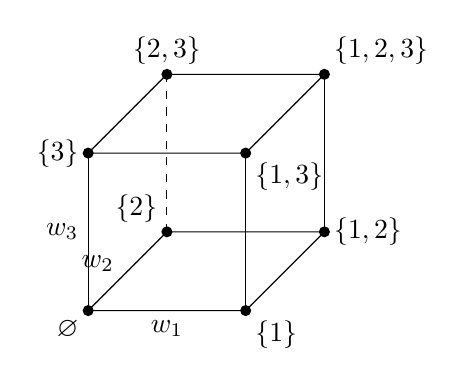
\begin{tikzpicture}[x=1cm,y=1cm]
					\coordinate (a) at (0,0);\coordinate (b) at (2,0);\coordinate (c) at (1,1);\coordinate (d) at (3,1);
					\coordinate (e) at (0,2);\coordinate (f) at (2,2);\coordinate (g) at (1,3);\coordinate (h) at (3,3);
					\draw (a)--node[below]{$w_1$}(b)--(d)--(c)--(a);
					\draw (e)--(f)--(h)--(g)--(e);
					\draw (a)--node[left]{$w_3$}(e);\draw (b)--(f);\draw[dashed] (c)--(g);\draw (d)--(h);
					\node[left] at (.45,.6) {$w_2$};
					\foreach \p in {a,b,c,d,e,f,g,h}\fill (\p) circle(2pt);
					\node[below left] at (a) {$\varnothing$};\node[below right] at (b) {$\{1\}$};
					\node[above left] at (c) {$\{2\}$};\node[right] at (d) {$\{1,2\}$};
					\node[left] at (e) {$\{3\}$};\node[below right] at (f) {$\{1,3\}$};
					\node[above] at (g) {$\{2,3\}$};\node[above right] at (h) {$\{1,2,3\}$};
				\end{tikzpicture}
			\end{adjustbox}
		\end{minipage}\hfill
		\begin{minipage}[c]{.51\textwidth}
			\centering
			\begin{tabular}{@{}r*{8}{r}@{}}
				\toprule $v\backslash u$&0&1&2&3&4&5&6&7\\\midrule
				0&--&--&--&--&--&--&--&--\\
				1&1&--&--&--&--&--&--&--\\
				2&1&0&--&--&--&--&--&--\\
				3&1&0&0&--&--&--&--&--\\
				4&1&0&0&1&--&--&--&--\\
				5&1&0&1&0&0&--&--&--\\
				6&1&1&0&0&0&0&--&--\\
				7&0&1&1&0&1&0&0&--\\\bottomrule
			\end{tabular}
		\end{minipage}
		\par\medskip
		$0:\varnothing,\ 1:\{1\},\ 2:\{2\},\ 3:\{1,2\},\ 4:\{3\},\ 5:\{1,3\},\ 6:\{2,3\},\ 7:[3].$
		\par\smallskip
		At each $w_i$: $\boxed{1}\;0\;0\;0$. The boxed cell pairs with each zero. The nine mixed pairs are
		\[
		\begin{array}{ll}
			w_1:&(1,0)\text{ with }(3,2),(5,4),(7,6),\\
			w_2:&(2,0)\text{ with }(3,1),(6,4),(7,5),\\
			w_3:&(4,0)\text{ with }(5,1),(6,2),(7,3).
		\end{array}
		\]
		\caption{The sharp three-cube construction. Vertex $I$ represents $x+\sum_{i\in I}w_i$ in binary coordinates. The strict-cell table and the mixed-pair lists use separated weights and the mask legend above. Each endpoint pair has a unique outer completion. The $1+3$ primitive splits give nine mixed corners. Table~\ref{tab:threecorners} in Appendix~\ref{app:verification} includes the other fifteen.}
		\label{fig:cube}
	\end{figure}

\subsection{Weak-source and cube certificates}
\paragraph{The four-by-four crop.}\label{app:crop-check}
We verify Table~\ref{tab:w1} and its inherited weak coloring by enumeration.

For fixed $d$, list the three colors at $(x,y),(x+d,y),(x+d,y+d)$ in lexicographic order of $(x,y)\in[4-d]^2$:
\begin{center}
	\begin{tabular}{@{}cl@{}}
		\toprule $d$&Complete list of color triples\\\midrule
		1&RGR, GRG, BGB, GBB, RBR, GRG, BGG, BGB, RBR\\
		2&RBR, GBG, GGB, RGR\\
		3&RGR\\\bottomrule
	\end{tabular}
\end{center}
None of the $9+4+1=14$ candidates is monochromatic. The six strict-source cells use only G and B, as required by the red diagonal. The inherited weak coloring $w_1(v,u)=f_4(v+1,u)$ has successive row words $\mathrm G$, $\mathrm{BB}$, and $\mathrm{GGB}$. Its diagonal classes are $\{1\}$ and $\{2,3\}$, both Golomb, although their union $F_1$ is not. The starts $1<2$ give the corner $(2,1),(3,1),(3,2)$ with colors G,B,B. For this example $M=6$, $L=3$, $T=\binom32+\binom22+\binom12=4$, and $E=4^2+2(3^2+2^2+1^2)=44$. 

The remaining tables verify Proposition~\ref{prop:74} and Theorems~\ref{thm:fourcube} and~\ref{thm:nine}.

\begin{table}[!htbp]
	\caption{Positive-offset verification of Table~\ref{tab:weak-rules}. Above, endpoints have color $c$ and completions have the last-column color. Below, $b_d,c_d$ count cells of color zero and one. Both panels are read from the array.}
	\label{tab:weak-completions}
	\centering
	\begin{tabularx}{\textwidth}{@{}rcp{.20\textwidth}Yc@{}}
		\toprule $d$&$c$&Starts&All pair completions&Color\\\midrule
		1&0&$\{7,12,21,22\}$&$(13,7),(22,7),(23,7),(22,12),(23,12),(23,21)$&1\\
		1&1&$\{0,4,23\}$&$(5,0),(24,0),(24,4)$&0\\
		2&1&$\{5,21\}$&$(23,5)$&0\\
		3&1&$\{1,4,21\}$&$(7,1),(24,1),(24,4)$&0\\
		4&0&$\{1,8\}$&$(12,1)$&1\\
		4&1&$\{0,4\}$&$(8,0)$&0\\
		5&0&$\{0,8\}$&$(13,0)$&1\\
		7&0&$\{1,5\}$&$(12,1)$&1\\
		8&0&$\{0,5,13\}$&$(13,0),(21,0),(21,5)$&1\\
		9&0&$\{4,13\}$&$(22,4)$&1\\
		11&1&$\{1,12\}$&$(23,1)$&0\\
		12&1&$\{0,12\}$&$(24,0)$&0\\
		16&1&$\{5,7\}$&$(23,5)$&0\\
		17&1&$\{4,7\}$&$(24,4)$&0\\\bottomrule
	\end{tabularx}\par\medskip
	\begin{tabular}{@{}rrrrr@{\qquad}rrrrr@{}}
		\toprule $d$&$r_d$&$b_d$&$c_d$&$\binom{r_d}{2}$&$d$&$r_d$&$b_d$&$c_d$&$\binom{r_d}{2}$\\\midrule
		1&7&4&3&21&13&2&1&1&1\\
		2&3&1&2&3&14&2&1&1&1\\
		3&4&1&3&6&15&2&1&1&1\\
		4&4&2&2&6&16&3&1&2&3\\
		5&3&2&1&3&17&3&1&2&3\\
		6&2&1&1&1&18&2&1&1&1\\
		7&3&2&1&3&19&2&1&1&1\\
		8&4&3&1&6&20&2&1&1&1\\
		9&3&2&1&3&21&2&1&1&1\\
		10&2&1&1&1&22&2&1&1&1\\
		11&3&1&2&3&23&2&1&1&1\\
		12&3&1&2&3&24&1&1&0&0\\\bottomrule
	\end{tabular}
\end{table}

\begin{table}[!htbp]
	\centering
	\caption{Exhaustive signed-support certificate for the four-cube. Internal $L,U$ words list the two parallel endpoints followed by the completion. Cross and bridge words list endpoint, completion, endpoint. The four family totals are $24,24,76,76$, and neither $000$ nor $111$ occurs.}
	\label{tab:fourtruth}
	\begin{tabular}{@{}lcl@{}}
		\toprule Family&$t$&Words and multiplicities\\\midrule
		$L$&1&001(3), 010(4), 011(2), 101(6), 110(3)\\
		$L$&2&011(3), 100(2), 110(1)\\
		$U$&1&001(3), 011(6), 100(6), 110(3)\\
		$U$&2&100(3), 101(3)\\
		$X$&1&001(7), 010(5), 011(8), 100(15), 101(4), 110(9)\\
		$X$&2&001(1), 010(9), 011(2), 100(5), 101(7)\\
		$X$&3&010(1), 011(1), 100(2)\\
		Bridge&1&001(6), 010(12), 011(6), 100(8), 101(12), 110(4)\\
		Bridge&2&010(5), 011(5), 100(6), 101(7), 110(1)\\
		Bridge&3&001(1), 100(1), 110(2)\\\bottomrule
	\end{tabular}
\end{table}

\begin{table}[!htbp]
	\centering
	\caption{The twenty-four three-cube corners. Words list $p,q,r$, with $q$ the outer completion. Bold M marks the nine mixed corners and F the forcing corners. Offsets are numerical values for weights $(1,3,9)$. Pairs use the mask legend in Figure~\ref{fig:cube}.}
	\label{tab:threecorners}
	\begin{tabular}{@{}rccclc@{\quad}rccclc@{}}
		\toprule $d$&$p$&$q$&$r$&Word&Type&$d$&$p$&$q$&$r$&Word&Type\\\midrule
		1&$(1,0)$&$(3,0)$&$(3,2)$&110&\textbf{M}&3&$(6,4)$&$(7,4)$&$(7,5)$&010&F\\
		1&$(1,0)$&$(5,0)$&$(5,4)$&110&\textbf{M}&4&$(3,0)$&$(7,0)$&$(7,4)$&101&F\\
		1&$(1,0)$&$(7,0)$&$(7,6)$&100&\textbf{M}&6&$(4,2)$&$(5,2)$&$(5,3)$&010&F\\
		1&$(3,2)$&$(5,2)$&$(5,4)$&010&F&8&$(4,1)$&$(6,1)$&$(6,3)$&010&F\\
		1&$(3,2)$&$(7,2)$&$(7,6)$&010&F&9&$(4,0)$&$(5,0)$&$(5,1)$&110&\textbf{M}\\
		1&$(5,4)$&$(7,4)$&$(7,6)$&010&F&9&$(4,0)$&$(6,0)$&$(6,2)$&110&\textbf{M}\\
		2&$(2,1)$&$(6,1)$&$(6,5)$&010&F&9&$(4,0)$&$(7,0)$&$(7,3)$&100&\textbf{M}\\
		3&$(2,0)$&$(3,0)$&$(3,1)$&110&\textbf{M}&9&$(5,1)$&$(6,1)$&$(6,2)$&010&F\\
		3&$(2,0)$&$(6,0)$&$(6,4)$&110&\textbf{M}&9&$(5,1)$&$(7,1)$&$(7,3)$&010&F\\
		3&$(2,0)$&$(7,0)$&$(7,5)$&100&\textbf{M}&9&$(6,2)$&$(7,2)$&$(7,3)$&010&F\\
		3&$(3,1)$&$(6,1)$&$(6,4)$&010&F&10&$(5,0)$&$(7,0)$&$(7,2)$&101&F\\
		3&$(3,1)$&$(7,1)$&$(7,5)$&010&F&12&$(6,0)$&$(7,0)$&$(7,1)$&101&F\\\bottomrule
	\end{tabular}
\end{table}

\FloatBarrier

\section{Examples of structured sources}\label{app:structured-examples}
\begin{remark}[Examples with repeated differences]\label{rem:structured-examples}
Put $D=\{0,1,3,4\}$ and $P=\{0,1\}$. The examples in Table~\ref{tab:structured-examples} all have repeated positive differences and proper strict two-colorings. The first two descriptions give the same set.
\begin{table}[htbp]
\centering
\caption{Finite examples for the structured families. The last column records the leading bound from Table~\ref{tab:structured}.}
\label{tab:structured-examples}
\small
\begin{tabular}{@{}llrrrcc@{}}
\toprule Family & Parameters & $n$ & $M$ & $T$ & $T/M$ & Bound\\\midrule
Progression & $B=D+9P$, $Q=27$, $t=2$ &16&120&200&$5/3$&$7/2$\\
Direct sum & $B=C=D$, $Q=9$ &16&120&200&$5/3$&$23/4$\\
Matching & $S=\{0,2\}$, $d=1$ &4&6&4&$2/3$&$10$\\
Two distances & $A=\{\pm1,\pm5,\pm25,\pm125\}$ &8&28&12&$3/7$&$6$\\
\bottomrule
\end{tabular}
\end{table}
For the first two rows, $A=D+9D$ is the cube with weights $1,3,9,27$. Table~\ref{tab:fourcube} gives a proper coloring. The separations are $27>2\cdot13$ and $9>2\cdot4$, and $E(A)=6^4=1296$, so $T(A)=200$.

For the matching $A=\{0,1,2,3\}$, read each row in increasing lower mark. The color words at upper marks $1,2,3$ are $0$, $01$, and $100$. The four corner words are $001$, $100$, $010$, and $010$. The translates interlace and their difference supports overlap: $E(A)=44$, whereas $E(S)E(\{0,1\})=36$. Thus separation is necessary for the product-energy identity.

The last row extends to $A_r=\{\pm5^i:0\le i<r\}$ for every $r\ge1$. Map $\pm5^i$ to $\pm e_i$, where the $e_i$ are orthonormal. In a pair-sum relation, the base-five coefficients have magnitude at most four, so the largest nonzero term cannot cancel. The map preserves all pair-sum equalities, and its nonzero squared distances belong to $\{2,4\}$.

Zero has $r$ unordered representations by antipodal pairs. Every nonzero pair sum has a unique unordered representation, including doubled marks. Therefore there are no three-term progressions and each pair of antipodal pairs gives two corners. Both have outer completion $(5^j,-5^j)$ for the four marks $-5^j<-5^i<5^i<5^j$. Coloring $(v,u)$ by one when $v=-u$ and zero otherwise is proper. Hence
\begin{equation}\label{eq:antipodal-counts}
|A_r|=2r,\quad M(A_r)=r(2r-1),\quad T(A_r)=r(r-1),\quad
\frac{T(A_r)}{M(A_r)}=\frac{r-1}{2r-1}\longrightarrow\frac12.
\end{equation}
The case $r=4$ gives the table entry. The supplementary verifier checks these colorings and counts.
\end{remark}

\begin{remark}[Asymptotic span comparison for matchings]
For a Golomb set of span at most $L$, Carter, Hunter, and O'Bryant~\cite{CHO25} give $|G|\le\sqrt L+\alpha L^{1/4}+O(1)$ with $\alpha=0.98183$. The two Golomb classes in Theorem~\ref{thm:matching} therefore give
\[
|S|\le2\sqrt L+2\alpha L^{1/4}+O(1),\qquad
M\le8L+16\alpha L^{3/4}+O(L^{1/2}).
\]
The leading coefficient eight follows already from classical Sidon estimates. This asymptotic estimate complements the finite bound \eqref{eq:matching-span} but is not used in the numerical Ramsey consequences.
\end{remark}

\section{\rev{Rainbow counts, counterexamples, and finite searches}}\label{app:rainbow-theory}
For $N\ge1$, let $\Ttri_N=\{(v,u):0\le u<v<N\}$. Write $\F_m(\rho)$ for the assertion that every proper three-coloring of $\Ttri_m$ has at least $\rho$ rainbow corners. A rainbow corner has three distinct colors. Counting equal-color pairs in rows, columns, and slope-one diagonals gives the following identity and upper bound.
\begin{lemma}[Three-color line identity]\label{lem:variance}
	In any three-coloring of $\Ttri_N$, let $\mathcal R_N,\mathcal B_N$ count rainbow and monochromatic corners. For its nonempty rows, columns, and slope-one diagonals $\lambda$, let $n_{\lambda,i}$ count color $i\in\{0,1,2\}$ and put
	\begin{equation}\label{eq:appendix-result-4}
\mathcal D_N=\sum_\lambda\sum_{i=0}^2(n_{\lambda,i}-|\lambda|/3)^2.
\end{equation}
	For every integer $N\ge1$,
	\begin{equation}\label{eq:appendix-result-5}
\mathcal D_N+2\mathcal R_N-4\mathcal B_N=N(N-1).
\end{equation}
	In particular, put $M_N=\binom N2$. A proper coloring satisfies $\mathcal D_N+2\mathcal R_N=N(N-1)$ and
	\begin{equation}\label{eq:appendix-result-6}
\mathcal R_N\le U_N:=M_N-(N-1)+\left\lfloor\frac{N-1}{3}\right\rfloor.
\end{equation}
\end{lemma}

\begin{proof}
	For a row pair $(v,u),(v,w)$ with $u<w<v$, its completion $(v-w+u,u)$ has first coordinate strictly between $u$ and $N$. For a column pair $(v,u),(w,u)$ with $u<v<w$, the completion $(w,u+w-v)$ has second coordinate between zero and $w-1$. For an offset pair $(u+d,u),(v+d,v)$ with $u<v$, the completion $(v+d,u)$ also remains in the triangle. Each pair direction fixes this unique completion, and no two directions describe the same distinct pair.
	
	The triangle has $\binom N3$ corners by Proposition~\ref{prop:counts}. A monochromatic corner contributes three equal-color pairs, a two-color corner one, and a rainbow none. Their total is therefore $P=\binom N3-\mathcal R_N+2\mathcal B_N$. Each line direction has one line of every length $1,\ldots,N-1$, so
	\[
	\sum_\lambda|\lambda|=3M_N,\quad
	\sum_\lambda|\lambda|^2=\frac{N(N-1)(2N-1)}2,\quad
	P=\frac{\mathcal D_N}{2}+\frac{N(N-1)(2N-1)}{12}-\frac{3M_N}{2}.
	\]
	The last equality follows by expanding $\sum_i\binom{n_{\lambda,i}}2$. Equate the expressions for $P$ and substitute $\binom N3=N(N-1)(N-2)/6$ to cancel the cubic terms and obtain the identity. At $N=1$, the line families are empty and every term is zero. Properness gives $\mathcal B_N=0$, and integrality sharpens $\mathcal D_N\ge0$ as follows. If two counts on a line differ by at least two, moving one unit from the larger count to the smaller decreases the sum of squares. Thus, for a line of length $\ell$, the minimum occurs when its three counts differ by at most one, and
	\[
	\sum_{i=0}^2(n_{\lambda,i}-\ell/3)^2\ge
	\begin{cases}
		0,&3\mid\ell,\\
		2/3,&3\nmid\ell.
	\end{cases}
	\]
	There are $(N-1)-\lfloor(N-1)/3\rfloor$ lengths not divisible by three, in each of the three directions. Hence
	\[
	\mathcal D_N\ge2\left((N-1)-\left\lfloor\frac{N-1}{3}\right\rfloor\right).
	\]
	Substitution into the identity gives $\mathcal R_N\le U_N$. The bound sums the line minima, which need not be attained simultaneously. The completion argument requires the full triangle and may fail for a sparse source.
\end{proof}

Assign a nonnegative weight to each dilation of a smaller triangle in $\Ttri_N$. A rainbow corner in the host may occur in several copies. Bounding the total weight of these occurrences controls the overcount.
\begin{lemma}[Weighted embedding implication]\label{lem:weighted}
	Fix integers $N\ge m\ge3$ and $\rho\ge0$. Assume $\F_m(\rho)$: every proper three-coloring of $\Ttri_m$ has at least $\rho$ rainbow corners. Let $a_d\ge0$ vanish outside $1\le d\le\lfloor(N-2)/(m-2)\rfloor$, and define
	\begin{equation}\label{eq:appendix-result-7}
J=\sum_d a_d\binom{N-d(m-2)}2,\qquad
	\Lambda_h=\sum_{\substack{j\mid h\\1\le j\le m-2}}\binom{m-j}2a_{h/j}.
\end{equation}
	If $K\ge0$ and $\Lambda_h\le K$ for $1\le h\le N-2$, then every proper three-coloring of $\Ttri_N$ satisfies $\rho J\le K\mathcal R_N\le KU_N$, where $U_N$ is defined in Lemma~\ref{lem:variance}. Thus, under $\F_m(\rho)$, the strict inequality $\rho J>KU_N$ implies $R_3(\Lconf)\le N$.
\end{lemma}

\begin{proof}
	Map $(v,u)\in\Ttri_m$ to $(u,v-u-1,m-1-v)$. These coordinates are nonnegative with sum $m-2$, and the inverse recovers $u,v$. A corner of step $j$ consists of a common nonnegative vector with $j$ added separately to each coordinate. Dilate by $d>0$ and add $(\alpha,\beta,\gamma)\ge0$ of sum $N-2-d(m-2)$. The physical map is
	\[
	\phi_{d,\alpha,\beta}(v,u)=(\alpha+\beta+1-d+dv,\ \alpha+du).
	\]
	The gap coordinates place the image in $\Ttri_N$. The map is injective and scales each positive step by $d$. A nonnegative triple summing to $q$ has $\binom{q+2}2$ choices, by placing two separators among $q$ identical units. Hence this dilation has exactly $\binom{N-d(m-2)}2$ labeled embeddings. Embeddings related by symmetry are counted separately.
	
	Under the stated local hypothesis, their weighted rainbow count is at least $\rho J$. Fix a host corner of step $h$. A local corner of step $j$ can map to it only at $d=h/j$, requiring $j\mid h$. If an embedding exists, its first cell uniquely fixes the two translation parameters. There are $\sum_{v=1}^{m-1-j}v=\binom{m-j}2$ local corners of step $j$. The host corner receives weight at most $\Lambda_h$, since boundary restrictions can only exclude embeddings. Sum over host rainbows and apply Lemma~\ref{lem:variance}. A proper $N\times N$ square restricts, after shifting indices by one, to a proper $\Ttri_N$, so impossibility of that triangle proves the Ramsey conclusion.
\end{proof}

\Needspace{6\baselineskip}
\begin{proposition}[Refutation of the two local rainbow bounds]\label{prop:local-rainbows}
	There is a proper three-coloring of $\Ttri_{11}$ with exactly three rainbow corners and a proper three-coloring of $\Ttri_{12}$ with exactly six. Consequently $\F_{11}(5)$ and $\F_{12}(7)$ are false.
\end{proposition}

\begin{proof}
Table~\ref{tab:local-rainbows} in Section~\ref{app:local-rainbow-certificates} gives all $55$ and $66$ cell colors. Enumerating each positive-step corner once gives zero monochromatic corners and respectively three and six rainbows. The table includes the enumeration rule and rainbow lists, giving counterexamples to both universal lower bounds.
\end{proof}

Section~\ref{app:failed-weights} gives weight certificates for these two refuted premises. The general embedding lemma applies to any valid local rainbow bound.

\begin{proposition}[Refutation of $\F_{13}(17)$]\label{prop:t13}
	There is a proper three-coloring of $\Ttri_{13}$ with exactly fourteen rainbow corners. Thus $\F_{13}(17)$ fails.
\end{proposition}
\begin{proof}
Table~\ref{tab:t13literal} in Section~\ref{app:t13certificate} assigns all $78$ cells and lists the fourteen zero-sum corners. The full sums in Table~\ref{tab:t13sums} enumerate all $286$ corners. Every zero-sum corner uses three distinct colors, and every other corner has nonzero sum modulo three and hence cannot be monochromatic. Thus the printed coloring is proper and has exactly fourteen rainbow corners.
\end{proof}

Whenever a proper three-coloring of $\Ttri_m$ exists, let
\[
r_m=\min_{c\text{ proper on }\Ttri_m}\mathcal R_m(c).
\]
The certificates give the upper bounds $r_{11}\le3$, $r_{12}\le6$, and $r_{13}\le14$. Establishing minima requires matching lower bounds, either by proof or by verifiable unsatisfiability certificates for smaller caps.

\begin{revision}
The next subsections give the complete counterexample certificates, followed by the rejected numerical weight argument and the SAT encoding. The counterexamples establish existence without claiming minimum rainbow counts or relying on unsatisfiability.
\end{revision}
\FloatBarrier

\subsection{\rev{Eleven- and twelve-mark certificates}}\label{app:local-rainbow-certificates}
	Row $v$ lists the colors of $(v,0),\ldots,(v,v-1)$ from left to right. The dash marks the absent row of $\Ttri_{11}$ at $v=11$.
	\begin{table}[!htbp]\centering\caption{Complete proper colorings for the eleven- and twelve-mark triangles.}\label{tab:local-rainbows}
		\begin{tabular}{@{}rll@{}}
			\toprule
			$v$ & $\Ttri_{11}$ & $\Ttri_{12}$\\\midrule
			1 & \texttt{2} & \texttt{1}\\
			2 & \texttt{20} & \texttt{01}\\
			3 & \texttt{201} & \texttt{100}\\
			4 & \texttt{0022} & \texttt{0011}\\
			5 & \texttt{10211} & \texttt{20121}\\
			6 & \texttt{220000} & \texttt{111000}\\
			7 & \texttt{0202020} & \texttt{0121110}\\
			8 & \texttt{11220111} & \texttt{22212222}\\
			9 & \texttt{212120001} & \texttt{121220202}\\
			10 & \texttt{1120120112} & \texttt{2210210201}\\
			11 & --- & \texttt{11011220012}\\
			\bottomrule
		\end{tabular}
	\end{table}
	For $m=11$ or $12$, every directed corner is obtained exactly once by taking $1\le d\le m-2$, $1\le v\le m-1-d$, and $0\le u<v$, then reading the colors of
	\[
	(v,u),\qquad(v+d,u),\qquad(v+d,u+d).
	\]
	Rows of lengths $1,\ldots,m-1$ specify all $\binom m2$ cell colors. Comparing entries for every permitted $(v,u,d)$ finds no monochromatic corner. In increasing step order, the rainbow counts are
	\[
	\begin{array}{ll}
		m=11:&(0,2,0,0,0,0,0,1,0),\\
		m=12:&(2,2,1,0,0,1,0,0,0,0).
	\end{array}
	\]
	The full rainbow lists, in the form $(v,u,d)$, are
	\[
	\begin{array}{ll}
		m=11:&(2,1,8),\ (6,3,2),\ (7,3,2),\\
		m=12:&(3,2,6),\ (6,3,2),\ (7,3,2),\ (8,4,3),\ (9,8,1),\ (10,1,1).
	\end{array}
	\]
	The enumeration covers $\sum_{d=1}^{m-2}\binom{m-d}{2}=\binom m3$ corners, namely $165$ and $220$. Every unlisted corner has two colors, so both colorings are proper with the stated rainbow counts.

\FloatBarrier

\subsection{\rev{The thirteen-mark certificate and corner sums}}\label{app:t13certificate}
\paragraph{Certificate for Proposition~\ref{prop:t13}.}
	Table~\ref{tab:t13literal} specifies every cell color $c(v,u)\in\mathbb F_3$ directly by its row word. For step $d>0$ define
	\[
	g_d(v,u)=c(v,u)+c(v+d,u)+c(v+d,u+d)\in\mathbb F_3.
	\]
	A triple sums to zero exactly when it is monochromatic or rainbow. These cases give $3a=0$ and $0+1+2=0$, whereas two copies of $a$ and a different color $b$ give $2a+b=b-a\ne0$.
	
	\begin{table}[htbp]
		\centering
		\caption{The coloring of $\Ttri_{13}$ and its zero-sum corners. Row $v$ lists colors at $u=0,\ldots,v-1$ in order. Each zero sum has the three distinct colors shown on the right. \rev{Table~\ref{tab:t13sums} lists all corner sums.}}\label{tab:t13literal}
		\begin{tabular}{@{}rl@{}}
			\toprule $v$&$c(v,0)\cdots c(v,v-1)$\\\midrule
			1 & \texttt{1} \\
			2 & \texttt{00} \\
			3 & \texttt{020} \\
			4 & \texttt{2022} \\
			5 & \texttt{21021} \\
			6 & \texttt{121000} \\
			7 & \texttt{2000202} \\
			8 & \texttt{21110021} \\
			9 & \texttt{121212210} \\
			10 & \texttt{1021221102} \\
			11 & \texttt{01122022111} \\
			12 & \texttt{010120120121} \\
			\bottomrule\end{tabular}\qquad
		\begin{tabular}{@{}rrc@{}}
			\toprule Base $(v,u)$&Step $d$&Colors $p,q,r$\\\midrule
			$(3,0)$ & 6 & $(0,1,2)$ \\
			$(4,2)$ & 2 & $(2,1,0)$ \\
			$(5,2)$ & 4 & $(0,1,2)$ \\
			$(5,2)$ & 5 & $(0,2,1)$ \\
			$(5,3)$ & 5 & $(2,1,0)$ \\
			$(6,0)$ & 1 & $(1,2,0)$ \\
			$(6,3)$ & 5 & $(0,2,1)$ \\
			$(6,4)$ & 5 & $(0,2,1)$ \\
			$(7,2)$ & 4 & $(0,1,2)$ \\
			$(7,5)$ & 2 & $(0,2,1)$ \\
			$(8,4)$ & 1 & $(0,1,2)$ \\
			$(8,4)$ & 2 & $(0,2,1)$ \\
			$(8,5)$ & 2 & $(0,2,1)$ \\
			$(8,6)$ & 2 & $(2,1,0)$ \\
			\bottomrule\end{tabular}\end{table}
	
	Table~\ref{tab:t13sums} lists every corner sum, ordered first by $d$, then by $v=1,\ldots,12-d$ and $u=0,\ldots,v-1$. Each of the $\binom{13}{3}=286$ corners occurs once. Table~\ref{tab:t13literal} lists exactly the zero entries and their colors.
	
	Every listed zero has three distinct colors, and every nonzero sum excludes monochromaticity. Thus the coloring is proper and its rainbow count is
	\[
	2+5+0+2+4+1+0+0+0+0+0=14<17.
	\]


\begin{table}[!htbp]
	\centering
	\caption{All $286$ corner sums modulo three. In step row $d$, slash-separated words run through base rows $v=1,\ldots,12-d$. Each word uses increasing $u$. The zero counts total fourteen, and Table~\ref{tab:t13literal} verifies every zero is rainbow.}\label{tab:t13sums}
	\begin{tabularx}{\textwidth}{@{}rYr@{}}
		\toprule $d$&Words by increasing base row&Zeros\\\midrule
		1 & \texttt{1} /\allowbreak \texttt{22} /\allowbreak \texttt{211} /\allowbreak \texttt{2112} /\allowbreak \texttt{21121} /\allowbreak \texttt{021222} /\allowbreak \texttt{2221222} /\allowbreak \texttt{21110122} /\allowbreak \texttt{211222122} /\allowbreak \texttt{2222112121} /\allowbreak \texttt{12221121211} & 2 \\
		2 & \texttt{1} /\allowbreak \texttt{12} /\allowbreak \texttt{221} /\allowbreak \texttt{1202} /\allowbreak \texttt{11222} /\allowbreak \texttt{112121} /\allowbreak \texttt{1121201} /\allowbreak \texttt{22210001} /\allowbreak \texttt{221121212} /\allowbreak \texttt{1212212121} & 5 \\
		3 & \texttt{2} /\allowbreak \texttt{12} /\allowbreak \texttt{111} /\allowbreak \texttt{1221} /\allowbreak \texttt{22122} /\allowbreak \texttt{121122} /\allowbreak \texttt{1212222} /\allowbreak \texttt{11221121} /\allowbreak \texttt{221122121} & 0 \\
		4 & \texttt{1} /\allowbreak \texttt{12} /\allowbreak \texttt{122} /\allowbreak \texttt{1121} /\allowbreak \texttt{12022} /\allowbreak \texttt{111221} /\allowbreak \texttt{1101212} /\allowbreak \texttt{12212121} & 2 \\
		5 & \texttt{2} /\allowbreak \texttt{22} /\allowbreak \texttt{222} /\allowbreak \texttt{2111} /\allowbreak \texttt{22002} /\allowbreak \texttt{121001} /\allowbreak \texttt{2221221} & 4 \\
		6 & \texttt{2} /\allowbreak \texttt{12} /\allowbreak \texttt{021} /\allowbreak \texttt{1112} /\allowbreak \texttt{11221} /\allowbreak \texttt{221211} & 1 \\
		7 & \texttt{1} /\allowbreak \texttt{22} /\allowbreak \texttt{221} /\allowbreak \texttt{1212} /\allowbreak \texttt{12121} & 0 \\
		8 & \texttt{2} /\allowbreak \texttt{12} /\allowbreak \texttt{112} /\allowbreak \texttt{2211} & 0 \\
		9 & \texttt{1} /\allowbreak \texttt{12} /\allowbreak \texttt{121} & 0 \\
		10 & \texttt{2} /\allowbreak \texttt{22} & 0 \\
		11 & \texttt{2} & 0 \\
		\bottomrule\end{tabularx}\end{table}

\FloatBarrier

\subsection{\rev{Divisor weights and load bounds}}\label{app:failed-weights}

The weights satisfy Lemma~\ref{lem:weighted}'s load constraints, but their local rainbow premises are false by Proposition~\ref{prop:local-rainbows}. The numerical gaps therefore yield no Ramsey improvement.

\FloatBarrier
\Needspace{7\baselineskip}
\begin{samepage}
\begin{proposition}[Integer weight certificates]\label{prop:weights}
	Take $N_{11}=459$ and $N_{12}=455$. For $m\in\{11,12\}$ put $c_j=\binom{m-j}2$ for $1\le j\le m-2$ and $K_m=1\,000c_1$, so $K_{11}=45\,000$, $K_{12}=55\,000$. Define successively
	\begin{equation}\label{eq:appendix-result-1}
a_n^{(m)}=\left\lfloor\frac{K_m-\sum_{\substack{j\mid n\\2\le j\le m-2}}c_j a_{n/j}^{(m)}}{c_1}\right\rfloor
	\quad(1\le n\le42),\qquad a_n^{(m)}=0\quad(n>42).
\end{equation}
	For $h\ge1$, define the divisor load $\Lambda_h^{(m)}=\sum_{j\mid h,\,1\le j\le m-2}c_j a_{h/j}^{(m)}$. All weights lie in $[0,1\,000]$, all positive-integer loads satisfy $\Lambda_h^{(m)}\le K_m$, and
	\begin{equation}\label{eq:appendix-result-2}
J_{11}=\sum_{d=1}^{42}a_d^{(11)}\binom{459-9d}2=944\,436\,978,\qquad
	J_{12}=\sum_{d=1}^{42}a_d^{(12)}\binom{455-10d}2=809\,226\,900.
\end{equation}
	These weight and load claims require neither local rainbow hypothesis.
\end{proposition}
\end{samepage}

\begin{proof}
	The local step coefficients are
	\[
	(c_j)_{11}=(45,36,28,21,15,10,6,3,1),\qquad
	(c_j)_{12}=(55,45,36,28,21,15,10,6,3,1).
	\]
	Table~\ref{tab:weights} gives all recurrence values and verifies that they lie in $[0,1\,000]$. For $h\le42$, the recurrence gives $0\le K_m-\Lambda_h^{(m)}<c_1$, so all these loads are within budget. For example the size-eleven recurrence at six has numerator $45\,000-36\cdot377-28\cdot200-10\cdot1\,000=15\,828$, giving $a_6=351$ and remainder $33$.
	
	Let $s(n)$ keep only the prime-power factors of $n$ drawn from $\{2,3,5,7\}$. Call $n$ smooth when $s(n)=n$. For $n\le42$, induction gives $a_n=a_{s(n)}$ for each weighting. Every allowed divisor $j>1$ uses only those four primes, so it divides $n$ exactly when it divides $s(n)$. Induction identifies the proper-divisor weights in the two recurrences, hence their floors. The claim is immediate for smooth $n$. When $s(n)=1$, the divisor sums are empty.
	
	For $m=11$, a nonsmooth $43\le h\le168$ has $s(h)\le15$, since its remaining factor is at least eleven. For $m=12$, the analogous range ends at $210$ and gives $s(h)\le19$. Every contributing $j$ divides $s(h)$. If $h/j\le42$, then $a_{h/j}=a_{s(h)/j}$. Adding the missing nonnegative terms, including the possibly absent $j=1$ term, gives $\Lambda_h\le\Lambda_{s(h)}\le K_m$.
	
	\rev{Table~\ref{tab:smooth} treats all remaining smooth integers} in the ranges $43\le h\le168$ for $m=11$ and $43\le h\le210$ for $m=12$. Enumerating $2^a3^b5^c7^e$ in these intervals gives the list, and the divisor formula gives each load. Together with the nonsmooth case, this covers the range between the small steps and the tail.
	
	For $m=11$, if $h\ge169$, a nonzero term requires $h/j\le42$, hence $j\ge5$. For $m=12$, if $h\ge211$, it requires $j\ge6$. In either case the sum of the remaining coefficients is $15+10+6+3+1=35$. Since every weight is at most $1\,000$,
	\[
	\Lambda_h^{(m)}\le35\,000<K_m.
	\]
	The load bound thus holds for every positive integer, even beyond the host. Substitution in \eqref{eq:appendix-result-2} gives both values of $J_m$.
\end{proof}

Put $M_N=\binom N2$ and $U_N=M_N-(N-1)+\lfloor(N-1)/3\rfloor$. Lemma~\ref{lem:variance} gives the rainbow interpretation of $U_N$.
\FloatBarrier
\Needspace{7\baselineskip}
\begin{proposition}[Arithmetic of a rejected numerical route]\label{thm:weighted}
	For the weights in Proposition~\ref{prop:weights}, the integer gaps are
\begin{equation}\label{eq:appendix-result-3}
5J_{11}-45\,000U_{459}=5\,959\,890>0,\qquad
7J_{12}-55\,000U_{455}=578\,300>0.
\end{equation}
The premises $\F_{11}(5)$ and $\F_{12}(7)$ would contradict these gaps by Lemma~\ref{lem:weighted}. Proposition~\ref{prop:local-rainbows} refutes both premises, so the gaps give no improvement for $R_3(\Lconf)$.
\end{proposition}

\begin{proof}
The largest dilation is $42$, and $42\cdot9\le459-2$ and $42\cdot10\le455-2$, so both weightings satisfy the support condition in Lemma~\ref{lem:weighted}. The definition gives
\[
U_{459}=105\,111-458+152=104\,805,\qquad
U_{455}=103\,285-454+151=102\,982.
\]
Substitute these values and the two values of $J_m$ from Proposition~\ref{prop:weights} to obtain the stated gaps. Under the respective local premise, Lemma~\ref{lem:weighted} would require each gap to be nonpositive. Proposition~\ref{prop:local-rainbows} supplies counterexamples to both premises.
\end{proof}


Tables~\ref{tab:weights} and~\ref{tab:smooth} give the weights and the remaining loads.

\begin{table}[!htbp]
\centering\small
\caption{All dilation weights. For each host, the copy-count factor is $C_d^{(m)}=\binom{N_m-d(m-2)}2$. Substitution in \eqref{eq:appendix-result-2} gives the two weighted totals. No local rainbow bound is assumed.}\label{tab:weights}
\begin{tabular}{@{}rrr@{\qquad}rrr@{\qquad}rrr@{}}
\toprule $d$&$a_d^{(11)}$&$a_d^{(12)}$&$d$&$a_d^{(11)}$&$a_d^{(12)}$&$d$&$a_d^{(11)}$&$a_d^{(12)}$\\\midrule
$1$ & $1000$ & $1000$ & $15$ & $459$ & $463$ & $29$ & $1000$ & $1000$ \\
$2$ & $200$ & $181$ & $16$ & $379$ & $382$ & $30$ & $118$ & $55$ \\
$3$ & $377$ & $345$ & $17$ & $1000$ & $1000$ & $31$ & $1000$ & $1000$ \\
$4$ & $373$ & $342$ & $18$ & $98$ & $94$ & $32$ & $419$ & $386$ \\
$5$ & $666$ & $618$ & $19$ & $1000$ & $1000$ & $33$ & $377$ & $345$ \\
$6$ & $351$ & $326$ & $20$ & $244$ & $218$ & $34$ & $200$ & $181$ \\
$7$ & $866$ & $818$ & $21$ & $410$ & $401$ & $35$ & $622$ & $575$ \\
$8$ & $541$ & $518$ & $22$ & $200$ & $181$ & $36$ & $323$ & $263$ \\
$9$ & $743$ & $719$ & $23$ & $1000$ & $1000$ & $37$ & $1000$ & $1000$ \\
$10$ & $400$ & $407$ & $24$ & $178$ & $131$ & $38$ & $200$ & $181$ \\
$11$ & $1000$ & $1000$ & $25$ & $778$ & $764$ & $39$ & $377$ & $345$ \\
$12$ & $266$ & $284$ & $26$ & $200$ & $181$ & $40$ & $393$ & $343$ \\
$13$ & $1000$ & $1000$ & $27$ & $529$ & $510$ & $41$ & $1000$ & $1000$ \\
$14$ & $280$ & $297$ & $28$ & $322$ & $278$ & $42$ & $258$ & $195$ \\
\bottomrule
\end{tabular}
\end{table}

\begin{table}[!htbp]
	\centering
	\caption{Remaining smooth-step loads for $43\le h\le168$ in the first weighting and $43\le h\le210$ in the second. Dashes lie beyond the first range, where the tail bound applies. Values are the divisor sums $\Lambda_h^{(m)}$.}\label{tab:smooth}
	\begin{tabular}{@{}rrr@{\quad}rrr@{\quad}rrr@{}}
		\toprule $h$&$\Lambda_h^{(11)}$&$\Lambda_h^{(12)}$&$h$&$\Lambda_h^{(11)}$&$\Lambda_h^{(12)}$&$h$&$\Lambda_h^{(11)}$&$\Lambda_h^{(12)}$\\\midrule
		$45$ & $24\,663$ & $33\,621$ & $84$ & $31\,310$ & $37\,306$ & $144$ & $9\,236$ & $11\,039$ \\
		$48$ & $29\,069$ & $37\,325$ & $90$ & $9\,764$ & $12\,839$ & $147$ & $2\,460$ & $4\,010$ \\
		$49$ & $5\,196$ & $8\,180$ & $96$ & $20\,058$ & $24\,998$ & $150$ & $9\,550$ & $13\,078$ \\
		$50$ & $34\,008$ & $43\,545$ & $98$ & $1\,680$ & $2\,970$ & $160$ & $15\,270$ & $19\,400$ \\
		$54$ & $29\,569$ & $38\,097$ & $100$ & $19\,998$ & $26\,377$ & $162$ & $5\,388$ & $7\,932$ \\
		$56$ & $23\,316$ & $30\,914$ & $105$ & $26\,320$ & $33\,751$ & $168$ & $10\,936$ & $13\,346$ \\
		$60$ & $28\,709$ & $35\,682$ & $108$ & $21\,399$ & $26\,010$ & $175$ & -- & $19\,715$ \\
		$63$ & $16\,804$ & $24\,080$ & $112$ & $9\,876$ & $13\,386$ & $180$ & -- & $7\,096$ \\
		$64$ & $24\,666$ & $31\,174$ & $120$ & $19\,969$ & $22\,971$ & $189$ & -- & $6\,303$ \\
		$70$ & $28\,992$ & $37\,000$ & $125$ & $11\,670$ & $16\,044$ & $192$ & -- & $6\,576$ \\
		$72$ & $24\,100$ & $29\,311$ & $126$ & $12\,192$ & $14\,866$ & $196$ & -- & $2\,780$ \\
		$75$ & $28\,669$ & $37\,227$ & $128$ & $9\,936$ & $13\,100$ & $200$ & -- & $12\,005$ \\
		$80$ & $26\,157$ & $32\,521$ & $135$ & $8\,394$ & $12\,099$ & $210$ & -- & $13\,671$ \\
		$81$ & $15\,555$ & $20\,517$ & $140$ & $19\,356$ & $24\,415$ &  &  &  \\
		\bottomrule\end{tabular}\end{table}

The SAT encoding below searches for finite counterexamples. S21 and G9 remain open.

\FloatBarrier

\subsection{SAT encoding}\label{app:sat}
Fix integers $n\ge3$ and $q\ge0$, and let $\mathcal H_n$ be the set of directed corners in $\Ttri_n$. There are $\binom n2$ cells and $\binom n3$ corners. To test a proposed lower bound $\F_n(q+1)$, we search for a proper three-coloring having at most $q$ rainbow corners. Introduce Boolean variables $x_{p,c}$ for $p\in\Ttri_n$ and $c\in\{0,1,2\}$, meaning that cell $p$ has color $c$. Impose
\[
\bigvee_{c=0}^2 x_{p,c},\qquad
\neg x_{p,c}\vee\neg x_{p,c'}\quad(c<c'),
\]
so each cell has exactly one color. For each corner $e=(p_1,p_2,p_3)$, impose
\[
\neg x_{p_1,c}\vee\neg x_{p_2,c}\vee\neg x_{p_3,c}
\quad(c=0,1,2),
\]
which forbids monochromatic corners. Introduce a Boolean variable $y_e$ and, for every permutation $\pi$ of $\{0,1,2\}$, impose
\[
\neg x_{p_1,\pi(0)}\vee\neg x_{p_2,\pi(1)}\vee
\neg x_{p_3,\pi(2)}\vee y_e.
\]
Every rainbow corner forces $y_e=1$. Finally impose the cardinality constraint
\[
\sum_{e\in\mathcal H_n}y_e\le q.
\]
The script \path{encode_rainbow_sat.py} turns this last constraint into clauses using a sequential counter~\cite{Sinz05} and exports a DIMACS formula together with a variable map. These implications for $y_e$ suffice: a satisfying assignment bounds the rainbow count by $q$, and any coloring within that cap extends to an assignment by taking $y_e$ as its rainbow indicator and setting the counter accordingly. The implementation also includes the three reverse clauses
\[
\neg y_e\vee x_{p_1,c}\vee x_{p_2,c}\vee x_{p_3,c}
\qquad(c=0,1,2),
\]
so $y_e$ is exactly the rainbow indicator. These clauses preserve every desired coloring. The default encoding uses no symmetry restriction.

\begin{table}[!ht]
	\centering\small
	\caption{The two satisfiable searches. Color-variable counts exclude rainbow indicators and counter variables. The final column comes directly from the colorings in Proposition~\ref{prop:local-rainbows}.}\label{tab:sat-targets}
	\begin{tabular}{@{}lrrrrr@{}}
		\toprule Assertion & Cells & Corners & Color variables & Cap $q$ & Actual rainbows\\\midrule
		$\F_{11}(5)$ & $55$ & $165$ & $165$ & $4$ & $3$\\
		$\F_{12}(7)$ & $66$ & $220$ & $198$ & $6$ & $6$\\\bottomrule
	\end{tabular}
\end{table}

The validator reconstructs the colors and checks every geometric corner. It finds no monochromatic corners and respectively three and six rainbows, verifying the assignments in Table~\ref{tab:sat-targets}. The assignments certify existence. They do not establish minimum rainbow counts or unsatisfiability below those counts.


\section{A general bound from the corners theorem}\label{sec:general}
The finite-abelian-group corners theorem of Jaber, Liu, Lovett, Ostuni, and Sawhney~\cite{JLLOS25} gives a general bound for $R_k(\Lconf)$. Reflection, paired colors, and a cyclic embedding handle the positive-step convention. All logarithms below are natural.

Write $\mathcal C(a,b;h)=\{(a,b),(a+h,b),(a,b+h)\}$ for a standard corner with integer step $h$.

\begin{lemma}[First-coordinate reflection]\label{lem:H}
	For integers $N,k\ge1$, put $\mathsf H_N(x,y)=(N+1-x,y)$. A coloring $\chi:[N]^2\to[k]$ avoids monochromatic positive directed L's if and only if $f=\chi\circ\mathsf H_N$ avoids monochromatic standard corners $\mathcal C(a,b;h)$ with $h>0$.
\end{lemma}
\begin{proof}
	Reflection sends $\Lconf(x,y;d)$ to $\mathcal C(N+1-x-d,y;d)$. Conversely, it sends $\mathcal C(a,b;d)$ to $\Lconf(N+1-a-d,b;d)$. Reflection is an involution of the square, so the formulas give both implications by pullback.
\end{proof}

\begin{lemma}[Half-turn and paired colors]\label{lem:J}
	Let $N,k\ge1$ be integers and let $f:[N]^2\to[k]$ avoid monochromatic positive standard corners. Put $\mathsf J_N(a,b)=(N+1-a,N+1-b)$ and $F(p)=(f(p),f(\mathsf J_Np))$. Then $F$ has at most $k^2$ colors, each class avoids standard corners of every nonzero integer step, and one class $S$ has $|S|\ge N^2/k^2$.
\end{lemma}
\begin{proof}
	A positive corner monochromatic for $F$ is monochromatic for its first component $f$. If the step $h$ were negative, its image under $\mathsf J_N$ would be a positive corner of step $-h$, monochromatic for $f$ by equality of the second components. Both cases contradict the hypothesis. At most $k^2$ ordered color pairs occur, so some class has at least $N^2/k^2$ cells.
\end{proof}

\begin{lemma}[Cyclic embedding without wraparound]\label{lem:embed}
	Let $N\ge1$ be an integer and let $S\subseteq[N]^2$ contain no standard corner of any nonzero integer step. Coordinate reduction $\iota:[N]^2\to G^2$, where $G=\Z/(2N\Z)$, is injective, and $\iota(S)$ has no group corner $(a,b),(a+\delta,b),(a,b+\delta)$ with $\delta\ne0$ in $G$.
\end{lemma}
\begin{proof}
	Reduction is injective because distinct elements of $[N]$ differ by less than $2N$. A group corner would therefore have representatives $(a,b),(a',b),(a,b')\in S$. The increments $h=a'-a$ and $t=b'-b$ satisfy $h\equiv t\pmod{2N}$, while
	\[
	|h-t|\le2N-2<2N.
	\]
	Thus $h=t$ as integers. Since the group step is nonzero, this common increment is nonzero. The three representatives give a forbidden integer corner in $S$.
\end{proof}

We use Theorem~1.1 of Jaber et al.~\cite{JLLOS25}, version~2, in the following finite-abelian-group form:
\begin{external}[Jaber et al., Theorem 1.1~\cite{JLLOS25}] There is an absolute $c>0$ such that every subset $A$ of the square of a finite abelian group $G$, avoiding standard group corners with nonzero step, satisfies
	\begin{equation}\label{eq:appendix-result-8}
|A|\le|G|^2\cdot\exp(-c(\log|G|)^{1/600}).
\end{equation}
\end{external}
Apply the theorem to $G=\Z/(2N\Z)$. Lemma~\ref{lem:embed} excludes every nonzero group step, as required.

\begin{theorem}[General bound from the external corners theorem]\label{thm:general}
	Fix an absolute constant $c>0$ valid in the cited external Theorem~1.1. Define
	\begin{equation}\label{eq:appendix-result-9}
B(k)=\left\lceil\exp\!\left(\left(\frac{\log(8k^2)}{c}\right)^{600}\right)\right\rceil,
	\qquad C=\left(\frac3c\right)^{600}.
\end{equation}
	For every integer $k\ge1$,
	\begin{equation}\label{eq:appendix-result-10}
R_k(\Lconf)\le B(k)\le\left\lceil\exp\!\bigl(C(\log(2k))^{600}\bigr)\right\rceil.
\end{equation}
	The external theorem supplies the constants, whose values are unspecified.
\end{theorem}

\begin{proof}
	Put $N=B(k)$ and suppose a proper $k$-coloring of $[N]^2$ exists. Lemmas~\ref{lem:H}--\ref{lem:embed} supply a class $S$ of size at least $N^2/k^2$ and its corner-free image in a group square of size $4N^2$. The external theorem gives
	\[
	\frac{N^2}{k^2}\le|S|\le4N^2\exp\!\left(-c(\log(2N))^{1/600}\right).
	\]
	The definition of $N$ and monotonicity on positive arguments give
	\[
	\log(2N)\ge\left(\frac{\log(8k^2)}c\right)^{600},\qquad
	c(\log(2N))^{1/600}\ge\log(8k^2).
	\]
	Thus $|S|\le4N^2/(8k^2)=N^2/(2k^2)<N^2/k^2$, contradicting the choice of $S$. Hence $R_k(\Lconf)\le B(k)$.
	
Since $8k^2\le(2k)^3$ for $k\ge1$,
\[
\left(\frac{\log(8k^2)}{c}\right)^{600}
\le C\bigl(\log(2k)\bigr)^{600}.
\]
Taking exponentials and ceilings proves the remaining bound.
\end{proof}

Hence $R_k(\Lconf)\le\exp(O((\log(2k))^{600}))$. This gives quasipolynomial dependence on $k$. The unspecified constant yields no new numerical bound for three or four colors.

\section{Sources and attribution}\label{app:provenance}
\begin{revision}
The Golomb input is the restriction used in~\cite[Theorem~6]{MSY25}:
same-color forced marks on a subdiagonal form a Golomb ruler. There,
length-dependent order bounds enter the interval count giving
$R_3(\Lconf)\le493$. Here Theorem~\ref{thm:energy} counts collisions
across two Golomb classes jointly and retains shared-difference and
class-size information. This refines the count on each $F_d(A)$.
A uniform estimate for the whole source is still needed to improve that
unconditional Ramsey bound.
\end{revision}

\begin{revision}
Wood~\cite[Lemmas~4,6--7]{Wood05} relates ordinary binary-vector pair
sums to common edge midpoints and gives the no-carry base-three
transfer to integer pair sums. Together with the known capacity
$a(4)=7$~\cite{OEIS309370}, this supplies the Sidon input used here.
Lemma~\ref{lem:capacity} proves the weighted upper bound directly. The
five-cube exclusion follows by combining this capacity with the inherited
coloring restriction. The four-cube construction and the sharp
three-cube mixed count additionally require one compatible coloring
of all source cells, which the capacity statement alone does not
provide.
\end{revision}

\begin{revision}
Musin~\cite{Musin09} uses regular-simplex edge midpoints to give the
standard two-distance set $\{e_i+e_j:i<j\}$, while Bannai et
al.~\cite{BSS12} study maximal few-distance extensions of Johnson
representations. Those questions concern geometric cardinality and
maximality. Here a pair-sum-preserving map transfers additive
relations into square counts, without assuming a common sphere.
For graph-selected simplex edges, the perfect-matching correspondence
gives $T(A_G)=2C_4(G)$. The complete-graph family and the limit
$T/M\to2$ follow directly from this correspondence. The underlying
geometric configuration is standard.
\end{revision}
\begin{revision}
The unrestricted energy maximum in Lemma~\ref{lem:small} is classical. Hegyv\'ari~\cite[Introduction]{Heg23} records the bound and its attainment by arithmetic progressions. We give a self-contained proof before deriving the endpoint deficit. The six-term progression exclusion reproduces a line-count argument referred to in the supplied revision record as coming from earlier research notes. The supplied materials do not identify the author, date or a retrievable version of those notes. Attribution therefore requires confirmation from the original records. The student does not claim this argument as an independent contribution. 
\end{revision}

Appendix~\ref{sec:general} uses Theorem~1.1 of the full version arXiv:2504.07006v2~\cite{JLLOS25}, dated 14 July 2025. The transfer to our orientation preserves the exponent $1/600$. SAT certificates are checked independently of search, following the practice in~\cite{HKM16}.

\section{Endpoint deletion}\label{app:endpoint}
Endpoint deletion gives exact local counts. The bounds below require an anchor condition, so the general assertion EP10 remains open.

\begin{lemma}[Exact endpoint deletion]\label{lem:deletion}
Let $A\subset\Z$ be finite and nonempty with $\min A=0$, and put $B=A\setminus\{0\}$. Define a directed graph $J_0(A)$ on $B$ by placing an arc $x\to w$ when $x<w$ and $w-x\in B$. Write $e_0(A)$ for its number of arcs, $D_0(A)$ for the number of additions $x+y=w$ with $x,y,w\in B$ and $0<x<y$, and $P_0(A)$ for the number of $x>0$ with $x,2x\in B$. Then
\begin{equation}\label{eq:endpoint-deletion}
T(A)-T(B)=e_0(A)=2D_0(A)+P_0(A).
\end{equation}
No coloring is required.
\end{lemma}
\begin{proof}
Zero cannot be the first coordinate of a strict cell. Each lost corner therefore has the unique form $(x,0),(w,0),(w,w-x)$ with $0<x<w$ and $x,w,w-x\in B$. These corners correspond bijectively to the arcs of $J_0(A)$. Distinct summands give two arcs and equal summands one. For empty $B$, there are no arcs. For deletion of the maximum $a$, the map $(v,u)\mapsto(a-u,a-v)$ identifies $V(A)$ with $V(a-A)$ and preserves positive corners and properness, giving the reflected identity.
\end{proof}

\begin{lemma}[A sharp restricted endpoint bound]\label{lem:anchor}
Let $|A|=n\ge2$ and $\min A=0$. Suppose a proper coloring $z:V(A)\to\{-1,1\}$ is \emph{all-forcing}, meaning that the parallel endpoints of every corner have equal signs. Put $B=A\setminus\{0\}$ and $f(a)=z(a,0)$ for $a\in B$. If all anchor signs equal $s$, then $e_0(A)=0$. If exactly one anchor $r\in B$ has sign $-s$, then $e_0(A)\le n-2$, with equality for arbitrarily large sources.
\end{lemma}
\begin{proof}
Any two cells in a difference fiber complete a corner, so the all-forcing hypothesis makes each fiber monochromatic. Thus $f$ extends to the represented positive differences and $z(v,u)=f(v-u)$. If $x,y,x+y\in B$, the corner $(x,0),(x+y,0),(x+y,y)$ gives $f(x+y)=-f(x)$. Interchanging the summands gives
\begin{equation}\label{eq:anchor-signs}
f(x)=f(y)=-f(x+y).
\end{equation}
This includes $f(2x)=-f(x)$ when $x=y$.

Uniform anchor signs exclude every such addition, proving $e_0=0$. If $r$ is the unique exceptional anchor, unequal summands must both be regular and sum to $r$. A doubling must have the form $2x=r$ or $r+r=2r$. Arcs ending at $r$ correspond to regular marks under $x\mapsto r-x$, so there are at most $n-2$. If $2r\in B$, that regular mark cannot participate in an addition ending at $r$, leaving at most $n-3$ such arcs and the one arc $r\to2r$. Thus $e_0\le n-2$.

For equality, take integers $k\ge1$ and $R\ge5$, and set
\begin{equation}\label{eq:endpoint-sharp-family}
x_0=0,\quad x_i=R^i\ (1\le i\le k),\quad r=R^{k+2},\qquad
A=\{x_i,r-x_i:0\le i\le k\}.
\end{equation}
The two groups of marks are disjoint and $|A|=2k+2$. In a relation between four marks, every base-$R$ coefficient has magnitude at most four. A largest nonzero term $R^j$ cannot be canceled because $4\sum_{i<j}R^i\le R^j-1$. Comparing coefficients therefore shows that the repeated positive differences are exactly
\begin{equation}\label{eq:endpoint-fibers}
\begin{array}{ccl}
\delta_{ij}=x_j-x_i&:&(x_j,x_i),\ (r-x_i,r-x_j),\\
h_{ij}=r-x_i-x_j&:&(r-x_j,x_i),\ (r-x_i,x_j),
\end{array}
\qquad 0\le i<j\le k.
\end{equation}
Each has the two displayed representations. The remaining differences $h_{ii}=r-2x_i$ occur once each. The list is exhaustive because every pair lies within one group or joins the two groups.

Color the fibers $\delta_{ij}$ and $h_{ij}$ by $s$ for $i<j$, and the fibers $h_{ii}$ by $-s$. The outer completion of either repeated fiber indexed by $i<j$ is $(r-x_i,x_i)$, with difference $h_{ii}$. Every corner is therefore proper and forcing. The anchor at $r$ is exceptional, while the anchors $x_i,r-x_i$ for $i>0$ have sign $s$. Coefficient uniqueness makes the positive additions exactly $x_i+(r-x_i)=r$ for $1\le i\le k$. They give $e_0=2k=n-2$.
\end{proof}
A two-mark source attains the zero bound. Restriction preserves the all-forcing property, but changing the minimum may invalidate the anchor condition in Lemma~\ref{lem:anchor}.

\begin{assertion}[EP10]\label{open:ep}
Every finite integer set $A$ with $|A|\ge2$ and properly two-colored $V(A)$ has an endpoint $a\in\{\min A,\max A\}$ such that
\begin{equation}\label{eq:ep10}
T(A)-T(A\setminus\{a\})\le10(|A|-1).
\end{equation}
\end{assertion}
\begin{assertion}[H10]\label{open:h}
Every finite integer set $A$ admitting a proper two-coloring of $V(A)$ satisfies $T(A)\le10M(A)$.
\end{assertion}

\begin{proposition}[Conditional endpoint reduction]\label{prop:peel}
Assume EP10. Then H10 holds and every properly two-colored strict source has $M\le21L$. For S21, it suffices to assume EP10 only on sources of span at most $99\,994$.
\end{proposition}
\begin{proof}
Each deletion preserves properness on the remaining cells. Iterate EP10 until one mark remains, using the translations and reflections of Lemma~\ref{lem:deletion}. The resulting sum telescopes:
\[
T(A)\le10\sum_{j=1}^{n-1}j=10M.
\]
Empty and singleton sources already have zero corners. Corollary~\ref{cor:span} gives $M\le21L$. Deletions never increase the span, proving the finite-range implication.
\end{proof}
EP10 and H10 remain open: iterating the restricted anchor estimate would require its hypothesis after every deletion.

\clearpage
\phantomsection\addcontentsline{toc}{section}{References}
\begingroup\small
% The bibliography is maintained in the accompanying references.bib file.
\bibliographystyle{plain}
\bibliography{references}
\endgroup
\end{document}
